%%%%%%%%%%%%%%%%%%%%%%%%%%%%%%%%%%%%%%%%%%%%%%%%%%%%%%%%%%%%%%%%%%%%%%%%%%%%%%%%%%%%%%%%%%%%%%%%%%%%%%%%%%%%%%%%
%BESCHREIBUNG
%%%%%%%%%%%%%%%%%%%%%%%%%%%%%%%%%%%%%%%%%%%%%%%%%%%%%%%%%%%%%%%%%%%%%%%%%%%%%%%%%%%%%%%%%%%%%%%%%%%%%%%%%%%%%%%%
%Autor (Vorlage): Janik Siller
%Created: 07/2018
%
% !TeX root = Projektarbeit.tex
%
%LaTeX Formatvorlage für wissenschaftliche Arbeiten
%
%Empfohlene LaTeX Distribution: TeXLive; 
%	Available: https://www.tug.org/texlive/
%Empfohlener Editor: Visual Studio Code; 
%	Available: https://code.visualstudio.com/
%Empfohlenes LaTeX Plugin für VS Code: LaTeX Workshop; 
%	Available: https://marketplace.visualstudio.com/items?itemName=James-Yu.latex-workshop
%
%Version: 2.0.2
%%%%%%%%%%%%%%%%%%%%%%%%%%%%%%%%%%%%%%%%%%%%%%%%%%%%%%%%%%%%%%%%%%%%%%%%%%%%%%%%%%%%%%%%%%%%%%%%%%%%%%%%%%%%%%%%

%%%%%%%%%%%%%%%%%%%%%%%%%%%%%%%%%%%%%%%%%%%%%%%%%%%%%%%%%%%%%%%%%%%%%%%%%%%%%%%%%%%%%%%%%%%%%%%%%%%%%%%%%%%%%%%%
%PRÄAMBEL
%%%%%%%%%%%%%%%%%%%%%%%%%%%%%%%%%%%%%%%%%%%%%%%%%%%%%%%%%%%%%%%%%%%%%%%%%%%%%%%%%%%%%%%%%%%%%%%%%%%%%%%%%%%%%%%%
\documentclass[
	pdftex,	
	a4paper,
	12pt,
	parskip = half,
	listof=totoc,
	bibliography=totoc,
    headheight = 50pt]
	{scrartcl}


% Sprachpaket Deutsch ------------------------------------------------------------------------------------------
\usepackage[ngerman]{babel}
% UTF8 und T1 Fontencoding -------------------------------------------------------------------------------------


\usepackage{csquotes}

\usepackage[backend=biber,style=alphabetic]{biblatex}

\addbibresource{content/literature.bib}

\usepackage[T1]{fontenc}
% ToDo Notes ---------------------------------------------------------------------------------------------------
%\usepackage{todonotes}
% Kopf / Fußzeilen----------------------------------------------------------------------------------------------
\usepackage[headsepline, footsepline]{scrlayer-scrpage}
% Grafiken einbinden--------------------------------------------------------------------------------------------
\usepackage{graphicx}
\usepackage{subcaption} % Benötigt für subfigure
\usepackage{listings}

% Einfache Verwendung von Farben -------------------------------------------------------------------------------
\usepackage{xcolor}
% Inhaltsverzeichnis als Lesezeichen in PDF --------------------------------------------------------------------
\usepackage{hyperref}
\hypersetup{hidelinks}
% Seitenränder -------------------------------------------------------------------------------------------------
\usepackage[left = 25mm, right=25mm, top=35mm, bottom=30mm, head=41pt]{geometry}
% Zeilenabstand ------------------------------------------------------------------------------------------------
\usepackage{setspace}
% Abkürzungen, Abkürzungsverzeichnis ---------------------------------------------------------------------------
\usepackage{acronym}
% Fixe Positionierung von Bildern mit der Option [H]------------------------------------------------------------
\usepackage{here}
% Latin Modern Schriftart - schönere Darstellung in PDF --------------------------------------------------------
\usepackage{lmodern}
% Mehr Darstellungsoptionen bei Aufzählungen -------------------------------------------------------------------
\usepackage{enumitem}
% Ermöglicht Berechnungen in den Argumenten von Kommandos ------------------------------------------------------
\usepackage{calc}
% Darstellung von Geburt und Tod -------------------------------------------------------------------------------
\usepackage{textcomp}
% Bessere Zeilentrennung zur Vermeidung von overful hbox -------------------------------------------------------
%\usepackage{microtype}
% AMS Mathematikpake--------------------------------------------------------------------------------------------
\usepackage{amsmath}
% Quellcodelistings --------------------------------------------------------------------------------------------
\usepackage{listings}
\usepackage{wrapfig}
\usepackage{textcomp}
\usepackage{textgreek}

%%%%%%%%%%%%%%%%%%%%%%%%%%%%%%%%%%%%%%%%%%%%%%%%%%%%%%%%%%%%%%%%%%%%%%%%%%%%%%%%%%%%%%%%%%%%%%%%%%%%%%%%%%%%%%%%
%META INFORMATIONEN
%%%%%%%%%%%%%%%%%%%%%%%%%%%%%%%%%%%%%%%%%%%%%%%%%%%%%%%%%%%%%%%%%%%%%%%%%%%%%%%%%%%%%%%%%%%%%%%%%%%%%%%%%%%%%%%%
% Projektspezifische Informationen -----------------------------------------------------------------------------
\newcommand{\titel}{Automatisiertes Modell-Hochregallager}
\newcommand{\arbeit}{T4-3100}
\newcommand{\studiengang}{Elektro- und Informationstechnik,\\Automation}
\newcommand{\hochschule}{DHBW Ravensburg}
\newcommand{\campus}{Campus Friedrichshafen}
\newcommand{\autor}{Thomas Martin und Melvin Zeuner}
\newcommand{\abgabe}{18.01.2027}
\newcommand{\zeitraum}{07.10.2026 - 18.01.2027}
\newcommand{\matrikelnummer}{2566504 und }
\newcommand{\kurs}{TEA 24}
\newcommand{\unternehmen}{DHBW Ravensburg, Campus Friedrichshafen}
\newcommand{\unternehmenstr}{}
\newcommand{\unternehmenaddr}{}
\newcommand{\betreuereins}{Prof. Dr. Ing. Thorsten Kever}
\newcommand{\betreuerzwei}{}
\newcommand{\betreuerdrei}{}
%\newcommand{\gutachter}{Prof. Dr. Gutachter}
\newcommand{\ort}{}
% Information für PDF Generierung ------------------------------------------------------------------------------
\hypersetup{
	pdftitle = {\titel},
	pdfsubject = {\titel},
	pdfauthor = {\autor}
}

%%%%%%%%%%%%%%%%%%%%%%%%%%%%%%%%%%%%%%%%%%%%%%%%%%%%%%%%%%%%%%%%%%%%%%%%%%%%%%%%%%%%%%%%%%%%%%%%%%%%%%%%%%%%%%%%
%LAYOUT
%%%%%%%%%%%%%%%%%%%%%%%%%%%%%%%%%%%%%%%%%%%%%%%%%%%%%%%%%%%%%%%%%%%%%%%%%%%%%%%%%%%%%%%%%%%%%%%%%%%%%%%%%%%%%%%%
%Kopf- und Fußzeilen -------------------------------------------------------------------------------------------
\pagestyle{scrheadings}
\clearpairofpagestyles
\ihead{
\includegraphics[height = 1.25 cm]{logos/logo_dhbw.png}}
\ohead{
\includegraphics[height = 0.65 cm]{logos/logo_rafi.png}}
\ofoot{\pagemark}
%Anpassen der KOMA Überschriften -------------------------------------------------------------------------------
\addtokomafont{sectioning}{\rmfamily}
%Zeilenabstand--------------------------------------------------------------------------------------------------
\onehalfspacing
%Counter für römische Seitenzahl -------------------------------------------------------------------------------
\newcounter{savepage}
%Quellenangabe von Grafiken ------------------------------------------------------------------------------------
\newcommand*{\quelle}[1]{\footnotesize ~#1}
%Größe von Abbildungen------------------------------------------------------------------------------------------
\newcommand{\imgsmall}{0.25\textwidth}
\newcommand{\imgmedium}{0.5\textwidth}
\newcommand{\imgbig}{0.75\textwidth}
\newcommand{\imglarge}{\textwidth}
%Quellcodeformatierung -----------------------------------------------------------------------------------------

%Farben------------------------------------
\colorlet{punct}{red!60!black}
\definecolor{background}{HTML}{EEEEEE}
\definecolor{delim}{RGB}{20,105,176}
\colorlet{numb}{magenta!60!black}
\definecolor{deepblue}{rgb}{0,0,0.5}
\definecolor{deepred}{rgb}{0.6,0,0}
\definecolor{deepgreen}{rgb}{0,0.5,0}

\DeclareFixedFont{\ttb}{T1}{txtt}{bx}{n}{8} % for bold
\DeclareFixedFont{\ttm}{T1}{txtt}{m}{n}{8}  % for normal

%JSON -------------------------------------
\lstdefinelanguage{json}{
	basicstyle=\scriptsize\normalfont\ttfamily,
    numbersep=8pt,
	showstringspaces=false,
	captionpos=b,
    breaklines=true,
    frame=lines,
    backgroundcolor=\color{background},
    literate=
     *{0}{{{\color{numb}0}}}{1}
      {1}{{{\color{numb}1}}}{1}
      {2}{{{\color{numb}2}}}{1}
      {3}{{{\color{numb}3}}}{1}
      {4}{{{\color{numb}4}}}{1}
      {5}{{{\color{numb}5}}}{1}
      {6}{{{\color{numb}6}}}{1}
      {7}{{{\color{numb}7}}}{1}
      {8}{{{\color{numb}8}}}{1}
      {9}{{{\color{numb}9}}}{1}
      {:}{{{\color{punct}{:}}}}{1}
      {,}{{{\color{punct}{,}}}}{1}
      {\{}{{{\color{delim}{\{}}}}{1}
      {\}}{{{\color{delim}{\}}}}}{1}
      {[}{{{\color{delim}{[}}}}{1}
      {]}{{{\color{delim}{]}}}}{1},
}
% Farben für die SCL-Syntax definieren
\definecolor{sclkeyword}{RGB}{0, 0, 255}   % Blau für Schlüsselwörter (IF, THEN, etc.)
\definecolor{sclstring}{RGB}{0, 0, 0}      % Schwarz für Variablen/Strings

% SCL-Sprache für listings definieren
\lstdefinelanguage{SCL}{
  keywords={IF, THEN, ELSIF, ELSE, END_IF, AND, OR, NOT, TRUE, FALSE},
  keywordstyle=\color{sclkeyword}\bfseries,
  sensitive=false,
  morecomment=[l]{//},
  morecomment=[s]{(*}{*)},
  morestring=[b]",
  morestring=[b]'
}

% Grundlegendes Aussehen der Codeblöcke festlegen
\lstset{
  language=SCL,
  basicstyle=\ttfamily\small,
  numbers=left,
  numberstyle=\tiny\color{gray},
  stepnumber=1,
  numbersep=6pt,
  frame=single,                % Einfacher Rahmen um den Code
  showstringspaces=false,
  tabsize=2,
  breaklines=true
}

%Python -------------------------------------
\newcommand\pythonstyle{\lstset{
    basicstyle=\scriptsize\normalfont\ttfamily,
    showstringspaces=false,
    language=Python,
	captionpos=b,
    breaklines=true,
    frame=lines,
    backgroundcolor=\color{background},
    otherkeywords={self},             % Add keywords here
    keywordstyle=\ttb\color{deepblue},
    emph={MyClass,__init__},          % Custom highlighting
    emphstyle=\ttb\color{deepred},    % Custom highlighting style
    stringstyle=\color{deepgreen},
    frame=tb                        % Any extra options here
}}

\lstnewenvironment{python}[1][]
{
\pythonstyle
\lstset{#1}
}
{}

%%%%%%%%%%%%%%%%%%%%%%%%%%%%%%%%%%%%%%%%%%%%%%%%%%%%%%%%%%%%%%%%%%%%%%%%%%%%%%%%%%%%%%%%%%%%%%%%%%%%%%%%%%%%%%%%
%HAUPTTEIL
%%%%%%%%%%%%%%%%%%%%%%%%%%%%%%%%%%%%%%%%%%%%%%%%%%%%%%%%%%%%%%%%%%%%%%%%%%%%%%%%%%%%%%%%%%%%%%%%%%%%%%%%%%%%%%%%

\begin{document}

    % Deckblatt ----------------------------------------------------------------------------------------------------
    \begin{titlepage}
	\vspace*{-\topskip}\vspace*{-\headsep}\vspace{-14mm}

	\begin{minipage}[c]{0.23\textwidth} 
    	
\includegraphics[height=1.25 cm]{logos/logo_dhbw.png} 
  	\end{minipage}
  	\hfill 
  	\begin{minipage}[c]{0.28\textwidth} 
    	 
\includegraphics[height=0.65 cm]{logos/logo_rafi.png}
  	\end{minipage}	
	
	\vspace{\headsep}\vspace{\topskip}
	
	\begin{center}		
		{\large \bfseries \titel}
		\vfill
		{\bfseries \arbeit}
		\vfill
		im Studiengang \studiengang
		\vfill
		an der \hochschule \\
		\campus
		\vfill
		von 
		\vfill
		\autor 
		\vfill
		\abgabe
		\vfill
	\end{center}
	
	\begin{tabular}{l l }
		Bearbeitungszeitraum: & \zeitraum \\
		Matrikelnummer: &    \matrikelnummer \\
		Kurs: &    \kurs \\
		Unternehmen: & \unternehmen \\
		& \unternehmenstr \\
		& \unternehmenaddr \\
		& \\
		Betreuer im Unternehmen: & \betreuereins \\
		& \betreuerzwei \\ & \betreuerdrei \\
		& \\
	%	Gutachter der Dualen Hochschule: & \gutachter \\
	
	\end{tabular}
	
\end{titlepage}

    % Eidesstattliche Erklärung-------------------------------------------------------------------------------------
    \newpage
    \pagenumbering{Roman}
    \section*{Eidesstattliche Erklärung} 


gemäß Ziffer 1.1.13 der Anlage 1 zu §§ 3, 4 und 5  der Studien- und Prüfungsordnung für die Bachelorstudiengänge 
im Studienbereich Technik der Dualen Hochschule Baden-Württemberg vom 29.09.2017 in der Fassung vom 25.07.2018.

Ich versichere hiermit, dass ich meine Projektarbeit mit dem Thema:
\begin{center}
{\bfseries \titel}
\end{center}
selbstständig verfasst und keine anderen als die angegebenen Quellen und Hilfsmittel benutzt habe. Ich 
versichere zudem, dass die eingereichte elektronische Fassung mit der gedruckten Fassung übereinstimmt.

\ort , den \abgabe .

\begin{tabular}{l}
\\
\\ \cline{1-1} 
{\footnotesize \autor} \hspace{15mm} \\

\end{tabular}

    % Sperrvermerk ------------------------------------------------------------------------------------------------
    \newpage
    \section*{Sperrvermerk} 
gemäß Ziffer 1.1.13 der Anlage 1 zu §§ 3, 4 und 5  der Studien- und Prüfungsordnung für die Bachelorstudiengänge 
im Studienbereich Technik der Dualen Hochschule Baden-Württemberg vom 29.09.2017 in der Fassung vom 25.07.2018:

{\bfseries \glqq Der Inhalt dieser Arbeit darf weder als Ganzes noch in Auszügen Personen außerhalb des 
Prüfungsprozesses und des Evaluationsverfahrens zugänglich gemacht werden, sofern keine anders lautende 
Genehmigung vom Dualen Partner vorliegt.\grqq}

\ort , den \abgabe .

\begin{tabular}{l}
\\
\\ \cline{1-1} 
{\footnotesize \autor} \hspace{15mm} \\

\end{tabular}

    %Leitgedanke ---------------------------------------------------------------------------------------------------
    %\newpage
    %\section*{Leitgedanke} 

\vfill
{\Large \itshape 
Man kann niemanden überholen, wenn man in seine Fußstapfen tritt}\\ \ \\
Francois Truffaut (\textborn 1932, \textdied 1984) %, franz. Biochemiker und Schriftsteller
\vfill

    %Kurzbeschreibung-----------------------------------------------------------------------------------------------
    \newpage
    \section*{Zusammenfassung} 
Diese Studienarbeit befasst sich mit der Weiterentwicklung eines automatisierten
Modell-Hochregallagers an der Dualen Hochschule Baden-Württemberg. Ziel ist es,
bestehende Funktionen um sichere und strukturierte Erweiterungen zu ergänzen und
das System stärker an industrielle Anforderungen anzupassen. Der Fokus liegt auf der
Integration einer sicherheitsgerichteten Lichtschranke, der Umsetzung eines internen
Umlagerungsprozesses sowie der Optimierung der SPS-Programmstruktur durch den
Einsatz der Programmiersprache Structured Text (ST). Die Lichtschranke wird über
IO-Link an eine Siemens S7-1500 angebunden und mithilfe geeigneter Prozesswerte
in die Sicherheitslogik integriert. Durch eine gezielte Auswertung des Prozesswertes
„Number of Beams Occupied“ kann der Gefahrenbereich zuverlässig überwacht und bei
unzulässigen Eingriffen eine automatische Abschaltung ausgelöst werden. Die Sicher
heitsfunktion ist vollständig in die bestehende Steuerungsarchitektur eingebettet und
mit dem Störungsmanagement gekoppelt. Ergänzend wird ein Umlagerungsprozess
realisiert, der die interne Verlagerung von Lagergütern ermöglicht. Eine eigenständige
Schrittkette stellt einen sicheren und flexiblen Ablauf des Prozesses sicher und berück
sichtigt sowohl die Bewegungslogik der Achsen als auch das Lagerplatzmanagement.
Insgesamt wird das Hochregallagersystem funktional, sicherheitstechnisch und struk
turell erweitert und bildet eine belastbare Grundlage für zukünftige, auftragsbasierte
Erweiterungen

    %Abstract-------------------------------------------------------------------------------------------------------
    \newpage
    \section*{Abstract} 
This study focuses on the further development of an automated model high-bay ware
house at the Baden-Wuerttemberg Cooperative State University. The objective is to
enhance existing functionalities by implementing safety-related and structural improve
ments and to align the system more closely with industrial automation requirements. Key
aspects of the work include the integration of a safety light curtain, the implementation of
an internal relocation process, and the optimization of the PLC program structure using
the programming language Structured Text (ST). The safety light curtain is connected
to a Siemens S7-1500 PLC via IO-Link and integrated into the control system using
selected process values. By evaluating the “Number of Beams Occupied” parameter, the
hazardous area can be reliably monitored and hazardous movements can be automati
cally stopped in the event of unauthorized access. The safety logic is fully embedded
into the existing control architecture and linked to the fault management system. In
addition, a relocation process is implemented to enable the internal transfer of load units
between different storage locations. A separate sequential control structure ensures
a safe and transparent process flow while taking into account axis movements and
storage location management. Overall, the high-bay warehouse system is significantly
improved in terms of functionality, safety, and software structure, providing a robust
foundation for future extensions such as order-based material flow control.

    %Danksagung-----------------------------------------------------------------------------------------------------
    %\newpage
    %\input{content/0_0_7Danksagung.tex}

    %Inhaltsverzeichnis---------------------------------------------------------------------------------------------
    \newpage
    \tableofcontents
    
    \setcounter{savepage}{\value{page}}
    \newpage

    %Beginn der Hauptkapitel-----------------------------------------------------------------------------------------------------
    \pagenumbering{arabic}
    \section{Einleitung}

\subsection{Motivation}

    

    
In Zeiten von \textbf{Industrie 4.0} hat die Bedeutung des Automatisierungsgrades in den
vergangenen Jahren erheblich zugenommen.
Besonders im Hinblick auf Effizienz, Sicherheit und die Effektivität automatisierter Abläufe spielt die Automatisierung eine zentrale Rolle.
Der Begriff \textbf{Industrie 4.0} beschreibt den aktuellen Wandel in der industriellen Pro
duktion hin zu intelligent vernetzten Systemen. Dabei spielt die Automatisierung eine
entscheidende Rolle. Die Kommunikation der einzelnen Maschinen, Produktionsanlagen
und Lager erfolgt hierbei über industrielle Netzwerke, was zu einem echtzeitfähigen
Verhalten beitragen kann.
Durch die zunehmende Digitalisierung und Vernetzung \textbf{industrieller Prozesse} entstehen
stetig neue Anforderungen an die Steuerungs- und Regelungstechnik. Diese Entwick
lungen führen zu immer komplexeren, aber auch effizienteren Produktions- und Logis
tiksystemen.


Gerade im Bereich der Lagerlogistik ist es entscheidend, sämtliche Sicherheitsmaß
nahmen einzuhalten, um einen reibungslosen und sicheren Ablauf zu gewährleisten.
Gleichzeitig wird eine präzise und fehlerarme Handhabung von Materialien ermöglicht,
was wesentlich zur Prozesssicherheit und Produktqualität beiträgt. Lagerprozesse sind
ein wesentlicher Bestandteil des Materialflusses innerhalb der Produktion. Fehler in
diesem Bereich können zu Stillständen und hohen Kosten führen. Um solche Probleme
zu vermeiden, ist ein reibungsloser Ablauf aller Prozessschritte erforderlich.

\subsection{Bedeutung der Lagerlogistik}
Im Bereich der Automatisierungstechnik existieren zahlreiche Konzepte, um Produkte
und Ersatzteile effizient zu lagern und zu verwalten.
Eine klassische Variante stellt die manuelle Lagerung in großen Lagerräumen dar.
Dabei sind jedoch umfangreiche Such- und Zuordnungsprozesse erforderlich, um die
gewünschten Komponenten zu identifizieren und zu entnehmen.
Eine wesentlich effektivere Lösung bietet die automatisierte Lagertechnik, insbesondere
das sogenannte „Hochregallager“.
Ein Hochregallager ermöglicht die automatisierte Ein- und Auslagerung von Materialien
und Ersatzteilen. Solche Systeme ermöglichen es durch den Einsatz moderner Sensorik,
wie etwa der Materialerkennung über \textbf{RFID} oder der automatischen Auftragsausführung
mittels QR-Code-Erkennung, Materialien präzise zu lagern und zu verwalten. Des Weiteren können die Prozesse über geeignete Softwarelösungen überwacht und gesteuert
werden.
Dadurch können Prozesszeiten verkürzt, Fehlerquoten reduziert und die Übersichtlich
keit innerhalb des Lagers deutlich verbessert werden.
Grundsätzlich lässt sich die Handhabung in zwei Varianten unterteilen:
• Automatische Ein- und Auslagerung
• Manuelle Ein- und Auslagerung
Das Hochregallager ist in der Regel in einem separaten Bereich installiert, in dem
autorisierte Mitarbeiter mithilfe eines Auftrags- oder Identifikationssystems auf die
eingelagerten Komponenten zugreifen können.
Die Automatisierung solcher Systeme ermöglicht eine zuverlässige, reproduzierbare
und sichere Abwicklung logistischer Prozesse. Hierdurch werden menschliche Fehler
weitestgehend reduziert und somit die Sicherheit erhöht

\subsection{Das DHBW-Hochregallager-Modell}
Zur Simulation und Demonstration der grundlegenden Lagerfunktionen wurde an der
Dualen Hochschule Baden-Württemberg (DHBW) eine Miniaturversion eines Hochre
gallagers entwickelt, die die wesentlichen Prozesse der Ein- und Auslagerung abbildet.
Das Modell eignet sich hervorragend als Lern- und Übungsplattform für Studierende,
um praxisnah Kenntnisse in der industriellen Automatisierung zu erwerben. Ziel des
Systems ist es, die Zusammenarbeit der einzelnen Sensoren und Aktoren zu simulieren
und dadurch den Studierenden einen praxisnahen Einblick in die industrielle Automati
sierung zu bieten.
Das System wurde in den vergangenen Jahren bereits mehrfach für Studien- und
Projektarbeiten im Studiengang „Elektrotechnik– Automation“ eingesetzt und kontinu
ierlich weiterentwickelt. Diese Arbeiten ermöglichten es den Studierenden, ein vertieftes
Verständnis für Steuerungs- und Automatisierungssysteme zu erlangen und praxisori
entierte Erfahrungen zu sammeln

\subsection{Zielsetzung der Studienarbeit}
Trotz der bisherigen Entwicklungen besteht weiterhin Verbesserungspotenzial, insbe
sondere im Bereich der Sicherheit und der Programmstruktur.
Die vorliegende Studienarbeit befasst sich daher mit der Überarbeitung und Einführung
neuer Sicherheitsmaßnahmen. Darüber hinaus soll eine auftragsbasierte Materialein
und-auslagerung implementiert werden. Weitere Schwerpunkte bilden die vollständige
Implementierung der \textbf{RFID}-basierten Materialerkennung sowie die Umstellung des
bestehenden SPS-Programms auf die Programmiersprache \textbf{Structured Text (ST)}.
Aufgrund des hohen Umfangs und der technischen Komplexität des Projekts erfolgt die
vollständige Umsetzung in den \textbf{Theoriephasen 5 und 6}.
Ziel der aktuellen Bearbeitung (Theoriephase 5) ist die Einführung neuer Sicherheits
konzepte und eines neuen Umlagerung- Prozesses.
Abschließend soll die durchgeführte Arbeit die Grundlage für die vollständige Realisie
rung eines funktionsfähigen, sicheren und didaktisch wertvollen Hochregallagermodells
bilden, das zukünftigen Studierenden als praxisnahes Lehr- und Forschungsobjekt
dient.
Die in den folgenden Kapiteln erläuterten Schritte zur Planung und Umsetzung sollen
verdeutlichen, wie die Studienarbeit (Teil 1) zur Weiterentwicklung der Funktionalität und
der Sicherheit des Systems beiträgt. Nun erfolgt eine Erläuterung der Problemstellung
und des aktuellen Standes der Technik
    \newpage
    \section{Grundlagen}
\subsection{Problemstellung}
Durch zahlreiche vorangegangene Studienarbeiten wurden bereits viele grundlegende
Funktionen des Hochregallagers implementiert.
Hierzu gehören unter anderem:

\begin{itemize}
    \item automatisiertes Einlagern,
    \item manuelles Auslagern,
    \item sowie die \textbf{RFID-Materialerkennung}.
\end{itemize}

Diese Funktionen bleiben im Rahmen dieser Arbeit bestehen und sind nicht Hauptbe
standteil der weiteren Bearbeitung.
Der Fokus der vorliegenden Studienarbeit liegt vielmehr auf der Integration zusätzlicher
\textbf{Sicherheitskomponenten}, der Fertigstellung der \textbf{RFID-Materialerkennung} sowie der
\textbf{Überarbeitung bzw. Umstellung des SPS-Programms} auf die Programmiersprache
\textbf{Structured Text (ST)}.
Für den sicheren Betrieb eines Hochregallagers sind verschiedene Schutzmecha
nismen erforderlich, um Gefahren beim Eingriff in den laufenden Prozess zu vermeiden.
Einige dieser Maßnahmen wurden bereits in früheren Arbeiten umgesetzt.
Ein wesentliches, bislang fehlendes Sicherheitselement ist jedoch eine Lichtschranke,
die sich unmittelbar vor dem Lagerbereich befindet. Diese soll im Rahmen dieser Arbeit
in das Steuerungsprogramm integriert werden, um potenzielle Gefährdungen bei manu
ellen Eingriffen während des Betriebs zu verhindern.


Darüber hinaus ist zur Gewährleistung eines fehlerfreien Ablaufs während der Ma
terialerkennung die Funktionalität der RFID-Prüfung zu analysieren, zu optimieren und
gegebenenfalls zu vervollständigen.
Ein weiterer wichtiger Aspekt betrifft die verwendete Programmiersprache des SPS
Systems. In den bisherigen Studienarbeiten wurde überwiegend die grafische Program
miersprache \textbf{FBS (Funktionsbausteinsprache)} eingesetzt. Diese bietet den Vorteil
einer einfachen, blockorientierten Programmstruktur, stößt jedoch bei komplexeren
Anwendungen schnell an ihre Grenzen.
Aus Gründen der Übersichtlichkeit, Wartbarkeit und Fehlersuche soll das bestehende
Programm daher in die textbasierte Programmiersprache \textbf{ST (Structured Text)} übertra
gen werden.
Abschließend lässt sich festhalten, dass die wesentlichen Funktionen des bestehenden
Hochregallagers bereits implementiert sind. Trotzdem bestehen noch Optimierungs
potenziale im Hinblick auf Sicherheit, Struktur und Programmiermethodik. Um die
geplanten Maßnahmen gezielt umsetzen zu können, ist es erforderlich, den aktuellen
technischen Aufbau und die bestehende Programmstruktur zunächst detailliert zu ana
lysieren. Im folgenden Abschnitt „Stand der Technik“ werden daher die vorhandenen
Komponenten und deren Funktion genauer betrachtet, um eine fundierte Grundlage für
die anschließende Überarbeitung zu schaffen

\subsection{Stand der Technik}
\subsubsection{Aufbau des Hochregallagers}
Bei der zu optimierenden Anlage handelt es sich um ein \textbf{Modell-Hochregallager} im
Laborraum H001 der \textbf{Dualen Hochschule Baden-Württemberg} am Campus Fried
richshafen. Diese dient dazu, den Studierenden bei vertretbaren Anschaffungskosten
ein Modell einer \textbf{modernen Hochregalanlage}, wie sie auch in zahlreichen \textbf{Industriebetrieben} zu finden ist, zu bieten.
Um den Aufbau der Anlage fachgerecht erklären zu können, ist die Definition eines
\textbf{Koordinatensystems} für die Bewegung der \textbf{Einlagerungsvorrichtung} notwendig:


\begin{figure}[H]
        \centering
        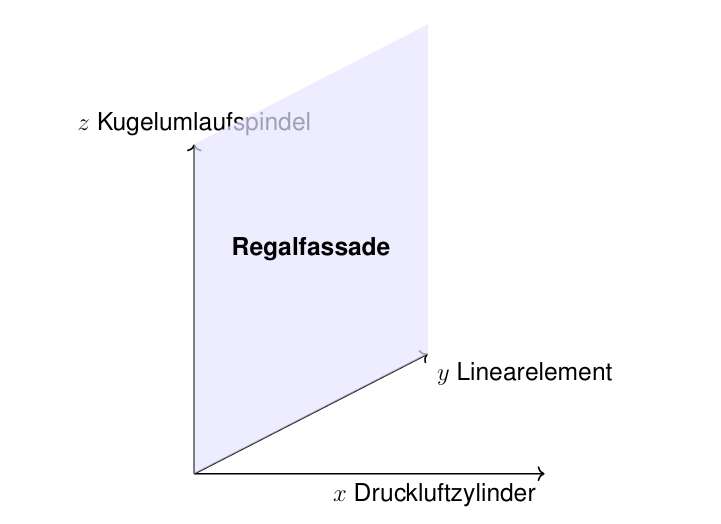
\includegraphics[width=400px]{images/KoordinatensystemAufbau.png}
        \caption{Schaubild zum Systemaufbau des Hochregallagers}
        \label{fig:koordsysaufbau}
    \end{figure}

\begin{itemize}
    \item x-Achse-> Bewegung des Trägers in das Hochregal
    \item y-Achse-> Bewegung des Trägers in Horizontale entlang der Regalstruktur
    \item z-Achse-> Bewegung des Trägers in Vertikale entlang der Regalstruktur
\end{itemize}




Die \textbf{Förder- und Bewegungssysteme} der Modell-Hochregalanlage stellen das zentrale
Element zur Realisierung \textbf{automatisierter Lagerprozesse} dar. Die Anlage ist so kon
zipiert, dass sie die \textbf{Ein- und Auslagerung} von Lagergütern in einem mehrstöckigen
Regalsystem ermöglicht. Die Bewegungsachsen werden in drei Dimensionen unterteilt:
\textbf{horizontal, vertikal} und die eigentliche \textbf{Einlagerbewegung}.


Die \textbf{horizontale Verfahrbewegung} (y-Achse) des Regalbediengeräts erfolgt über ein
\textbf{Linearelement}, das entlang einer \textbf{Führungsschiene} verläuft. Das Linearsystem basiert
auf einem \textbf{motorgetriebenen Schlitten}, welcher präzise Positionierungen entlang der
Regalfassade ermöglicht. Die Führungsschiene gewährleistet eine stabile und reibungs
arme Bewegung, während der Antrieb über einen \textbf{Schrittmotor} erfolgt, der über eine
\textbf{Steuerungseinheit} angesteuert wird. Die Positionserfassung wird gegenwärtig durch
\textbf{Timer im Steuerungsprogramm} realisiert. Die Positionierung der \textbf{Endschalter} erfolgt
ausschließlich am Ende der Achsen.


Die \textbf{vertikale Bewegung} (z-Achse) wird durch eine \textbf{Kugelumlaufspindel} realisiert,
die eine hohe Positioniergenauigkeit und mechanische Effizienz bietet. Die Spindel ist
mit einem \textbf{rotatorischen Antrieb} gekoppelt, der die Drehbewegung in eine lineare
\textbf{Hubbewegung} umsetzt. Die Verwendung von \textbf{Kugelumlaufmuttern} führt zu einer
Minimierung der Reibung und einer Erhöhung der Tragfähigkeit, was insbesondere bei
mehrstöckigen Regalsystemen vorteilhaft ist. 
Die vertikale Führung erfolgt über ein sta
biles Profil, das die Bewegung des Hubsystems stabilisiert und ein Verkanten verhindert.



Die eigentliche \textbf{Einlagerung des Lagerguts} (x-Achse) erfolgt mittels eines \textbf{Druck
luftzylinders}. Der Zylinder ist am Regalbediengerät montiert und fährt bei Erreichen
der Zielposition aus, um das Lagergut in das vorgesehene Fach zu überführen. Die
Wahl eines pneumatischen Systems ermöglicht eine schnelle und kraftvolle Bewegung,
die unabhängig von der elektrischen Steuerung arbeitet und sich gut für wiederholte,
gleichförmige Bewegungsabläufe eignet. Die Steuerung des Zylinders erfolgt durch ein
\textbf{Magnetventil}, das durch die SPS angesteuert wird.
Die \textbf{Sensorik und Steuerungseinheiten} der Modell-Hochregalanlage übernehmen
zentrale Aufgaben zur Gewährleistung eines sicheren und präzisen Betriebs. Sie er
möglichen sowohl die \textbf{Positionsbestimmung} der beweglichen Komponenten als auch
die \textbf{Identifikation der Lagergüter} und die \textbf{Prozesssteuerung}.
Zur Erfassung der Endstellungen der horizontalen und vertikalen Bewegungsachsen
werden mechanische \textbf{Endschalter} verwendet. Diese sind jeweils an den Begrenzungs
punkten der Lineareinheit sowie der Kugelumlaufspindel angebracht und dienen der
sicheren Detektion der maximalen Verfahrwege. Das Erreichen einer Endlage löst
den entsprechenden Schalter aus und führt zur Übertragung eines Signals an die
Steuerungseinheit. Diese Vorgehensweise verhindert ein Überfahren der mechanischen
Grenzen und gewährleistet den Schutz der Anlage vor potenziellen Schäden.



Die \textbf{Materialerfassung} erfolgt mittels eines \textbf{RFID-Systems}, welches sich aus einer
\textbf{RFID-Antenne} und entsprechenden \textbf{Transpondern} zusammensetzt. Jedes Element
des Lagers ist mit einem \textbf{RFID-Tag} ausgestattet, der eine eindeutige Identifikation
ermöglicht. Die Positionierung der Antenne erlaubt es, beim Ein- oder Auslagern eines
Artikels dessen Transponder auszulesen. Die erfassten Daten werden unmittelbar an die
Steuerung übermittelt und dort verarbeitet. Das berührungslose Identifikationsverfahren
ermöglicht eine schnelle und fehlerfreie Zuordnung der Lagergüter.



Die zentrale Steuerung der Anlage erfolgt mittels einer \textbf{SPS vom Typ Siemens S7-1511},
welche sämtliche Bewegungsabläufe, Sensorrückmeldungen und Aktorsteuerungen
koordiniert. Die SPS ist über ein \textbf{HMI (Human-Machine Interface)} mit dem Bedienper
sonal verbunden, wodurch eine intuitive Bedienung und Visualisierung der Anlagenzu
stände ermöglicht wird. Über das HMI können Betriebsmodi gewählt, Lagerprozesse
gestartet und Diagnosedaten eingesehen werden.




\subsubsection{Speicherprogrammierbare Steuerungen}
Die \textbf{Speicherprogrammierbare Steuerung} (SPS) stellt ein zentrales Element moderner
industrieller Automatisierung dar.Sie ermöglicht die flexible, softwarebasierte Steuerung
technischer Prozesse und ersetzt zunehmend klassische \textbf{verbindungsprogrammierte
Steuerungen} wie Relais-und Schütztechnik. Insbesondere die SPS-Systeme der
Siemens AG, unter dem Markennamen SIMATIC bekannt, nehmen eine führende Rolle
in der industriellen Praxis ein.
Im folgenden eine Gegenüberstellung von VPS und SPS:

\begin{center}
    % Erzeugt eine normale Tabellenbeschriftung ohne \begin{table}

    \begin{tabular}{|p{4cm}|p{6cm}|p{6cm}|}
        \hline
            \textbf{Kriterium}  & \textbf{SPS (Speicherprogrammierbare Steuerung)} & \textbf{VPS (Verbindungsprogrammierte Steuerung)} \\
            \hline
            \textbf{Flexibilität}& Hohe Flexibilität durch einfache Softwareänderung& Geringe Flexibilität,Änderungen erfordern Hardwareeingriffe\\
            \hline
            \textbf{Programmierung} &  Softwarebasiert über Programmiersprachen(z.B.KOP, FUP,SCL)& Hardwarebasiert durch Verdrahtung von Relais und Schützen\\
            \hline
            \textbf{Fehlersuche}& Komfortable Diagnosefunktionen über Softwaretools& Fehlersuche oft manuell und zeitaufwendig\\
            \hline
            \textbf{Platzbedarf}& Kompakte Bauweise, platzsparend & Großer Platzbedarf durch viele Einzelkomponenten\\
            \hline
            \textbf{Kosten bei Änderungen}& Geringe Kosten, da keine Hardwareänderungnötig& Hohe Kosten durch Umbau und neue Komponenten\\
            \hline
            \textbf{Wartung}&Zentralisiert und soft waregestützt& Dezentral und hardwareintensiv  \\
            \hline
            \textbf{Komplexität der Steuerung}& Geeignet für komplexe und vernetzte Systeme & Nur für einfache Steuerungsaufgaben geeignet   \\
            \hline
            \textbf{Zukunftsfähigkeit}& Industrie 4.0-fähig, IoT-Integration möglich & Veraltet,kaum kompatibel mit modernen Systemen \\
            \hline
    \end{tabular}

    \captionof{table}{Vergleich zwischen SPS und VPS hinsichtlich technischer und wirtschaftlicher Kriterien; Quelle:[21]}
    \label{tab:VergleichSpsVps}
\end{center}


Die SIMATIC-Reihe von Siemens ist in zwei Produktlinien gegliedert,welche sich
hauptsächlich in ihren Anwendungsbereichen unterscheiden. Die S7-1200 ist für die
Realisierung kompakter Automatisierungslösungen konzipiert,wohingegen die S7-1500
erweiterte Funktionen für die Bewältigung komplexer Steuerungsaufgaben in vernetzten
Produktionsumgebungen bietet. Die Funktionsweise beider Systeme ist durch das
EVA-Prinzip (Eingabe– Verarbeitung– Ausgabe) determiniert. Die Bereitstellung der
Eingangssignale erfolgt durch Sensoren, deren Signale durch die CPU verarbeitet und
anschließend durch Aktoren umgesetzt werden


\begin{figure}[H]
        \centering
        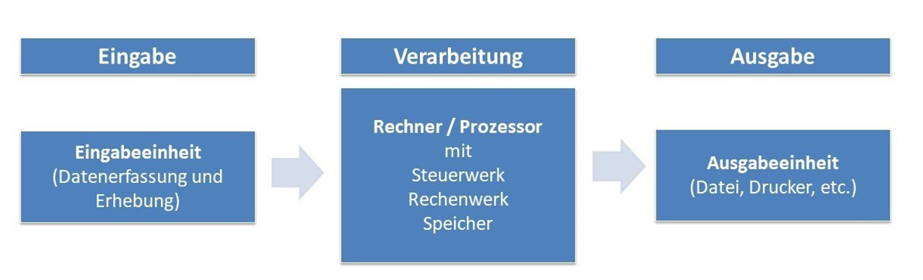
\includegraphics[width=\textwidth]{images/EVAPrinzip.png}
        \caption{EVA-Prinzip; Quelle [20]}
        \label{fig:eva}
    \end{figure}


Die Programmierung und Konfiguration der Siemens-SPS erfolgt über das \textbf{Totally Inte
grated Automation Portal} (TIA Portal), eine integrierte Entwicklungsumgebung, die
verschiedene Automatisierungskomponenten wie SPS, HMI und Antriebstechnik vereint.
Das TIA Portal unterstützt die Programmiersprachen gemäß \textbf{IEC 61131-3}, darunter
\textbf{Kontaktplan} (KOP), \textbf{Funktionsplan} (FUP), \textbf{Anweisungsliste} (AWL) und \textbf{Structured
Control Language} (SCL). Diese Vielfalt ermöglicht eine anwendungsorientierte und
normgerechte Entwicklung von Steuerungsprogrammen.[12]

    \begin{figure}[H]
        \centering
        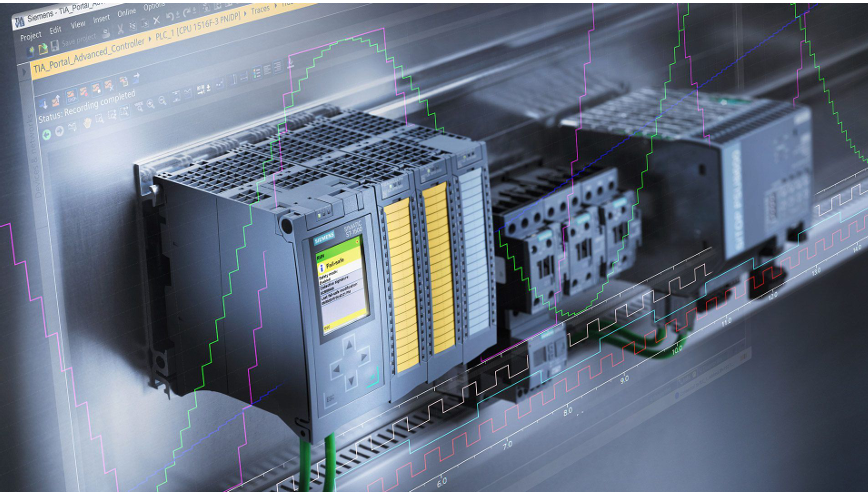
\includegraphics[width=\textwidth]{images/S7-1500.png}
        \caption{Beispiel S7-1500; Quelle [19]}
        \label{s7-1500}
    \end{figure}

Ein wesentliches Merkmal der \textbf{Siemens-SPS-Systeme} ist ihre Kompatibilität mit modernen Kommunikationsstandards wie \textbf{PROFINET} und \textbf{PROFIBUS}. Dadurch wird ei
ne nahtlose Integration in industrielle Netzwerke gewährleistet. Im Kontext von \textbf{Industrie 4.0} kommt den Siemens-SPS eine Schlüsselrolle zu, da sie die Grundlage
für intelligente, vernetzte und adaptive Produktionssysteme bilden. Die Fähigkeit zur
\textbf{Echtzeit-Datenerfassung und-verarbeitung} sowie zur Anbindung an Cloud- und
\textbf{IoT-Plattformen} macht sie zu einem integralen Bestandteil digitalisierter Fertigungspro
zesse.[22

\subsubsection{SPS-Programmierung}
In der Automatisierungstechnik werden speicherprogrammierbare Steuerungen (SPS)
zur Realisierung unterschiedlichster Abläufe eingesetzt. Um die gewünschten Funktio
nen zur Automatisierung von Prozessen umzusetzen, ist es erforderlich, diese Abläufe
in Form eines Programms in die Steuerung zu implementieren.
Ein SPS-Programm folgt dabei in der Regel einem klar strukturierten Aufbau [16]:

\begin{itemize}
    \item Definition der Ein-, Ausgangs- und Hilfsvariablen in einer Variablentabelle,
    
    \item Programmierung des Hauptprogramms mit den zugehörigen Unterprogrammen und Funktionsbausteinen,

    \item Kompilierung des Programms und Übertragung in die Steuerung.
\end{itemize}


    \begin{figure}[H]
        \centering
        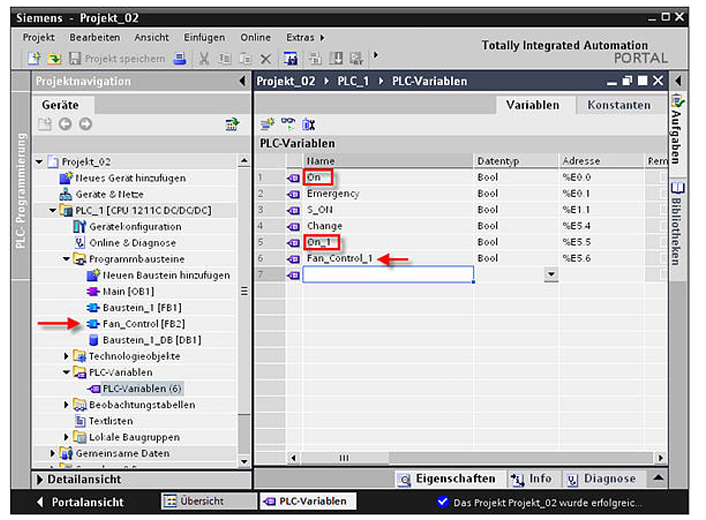
\includegraphics[width=\textwidth]{images/VariablentabelleTIA.png}
        \caption{Übersicht der Variablentabelle in TIA Portal [18]}
        \label{vartabtia}
    \end{figure}


Das Hauptprogramm besteht aus sogenannten \textbf{POUs} (Program Organization Units,
deutsch: Programmorganisationseinheiten). Diese werden in drei Arten unterteilt: \textbf{Pro
gramme}, \textbf{Funktionen} (FC) und \textbf{Funktionsbausteine} (FB). Die Realisierung dieser
POUs in Siemens TIA Portal wurde bereits im vorherigen Kapitel \ref{XXXXXXXXX} beschrieben.

Nachfolgend wird die Bedeutung und Funktion der einzelnen Organisationseinheiten
erläutert.


Das \textbf{Programm} dient der Realisierung komplexer Abläufe, beispielsweise von Schrittket
ten oder Hauptlogiken. Eine \textbf{Funktion} (FC) ist mit einer C-ähnlichen Funktion vergleich
bar. Sie verarbeitet eine oder mehrere Eingangsvariablen und gibt nach der Abarbeitung
ein Ergebnis zurück. Gemäß IEC 61131-3 können Funktionen jedoch nicht rekursiv
aufgerufen werden und besitzen kein eigenes Speicherverhalten, d.h. sie können kei
ne Werte dauerhaft speichern [16]. Ein einfaches Beispiel hierfür ist ein logisches
\textbf{UND-Gatter}.
Ein \textbf{Funktionsbaustein} (FB) hingegen besitzt ein internes Gedächtnis und kann Werte
über mehrere Zyklen hinweg speichern. Dadurch eignet er sich besonders für Zu
standsautomaten oder speichernde Operationen. Ein klassisches Beispiel hierfür ist ein
\textbf{RS-Flip-Flop}.


Für die Programmierung stehen verschiedene Sprachen nach IEC 61131-3 [1] zur
Verfügung:

\begin{itemize}
    \item \textbf{KOP} (Kontaktplan),
    \item \textbf{AWL} (Anweisungsliste),
    \item \textbf{FUP/FBS} (Funktionsplan / Funktionsbausteinsprache),
    \item \textbf{ST/SCL} (Structured Text / Structured Control Language)1
\end{itemize}


In modernen Industrieanlagen werden überwiegend FUP und ST eingesetzt. Diese
Programmiersprachen zeichnen sich durch eine gute Übersichtlichkeit und eine effizi
ente Fehleranalyse aus. Trotzdem bestehen zwischen beiden Varianten wesentliche
Unterschiede, die in Tabelle 2 dargestellt sind.


\begin{center}
    % Erzeugt eine normale Tabellenbeschriftung ohne \begin{table}

    \begin{tabular}{|p{6cm}|p{6cm}|}
        \hline
            \textbf{ST / SCL (Structured Text / Structured Control Language)}  & \textbf{FUP (Funktionsplan)}\\
            \hline
            Textbasierte Programmiersprache & Grafische Programmiersprache\\
            \hline
            Hochsprachenähnlich (z.B. C, Pascal) & Verwendung grafischer Symbole und logischer Verknüpfungen\\
            \hline
            Klare und kompakte Struktur & Gefahr der Unübersichtlichkeit bei komplexen Programmen\\
            \hline
            Besonders geeignet für mathematische und logische Operationen & Gut geeignet für einfache logische Abläufe\\
            \hline
    \end{tabular}

    \captionof{table}{Vergleich zwischen ST (Structured Text) und FUP (Funktionsplan) [17]}
    \label{tab:VergleichSclFup}
\end{center}


1 \textbf{SCL} ist die Siemens-spezifische Implementierung der nach IEC 61131-3 genormten Programmierspra
che Structured Text (ST) im TIA Portal [13].
\ref{XXX}



Wie aus der Tabelle hervorgeht, bietet die textbasierte Programmiersprache \textbf{ST} ins
besondere bei komplexen Strukturen und mathematischen Berechnungen erhebliche
Vorteile. \textbf{FUP} hingegen ist für Einsteiger leichter verständlich und eignet sich für über
schaubare Steuerungslogiken. Mit zunehmender Komplexität der Abläufe stößt FUP
jedoch schnell an seine Grenzen, da die grafische Darstellung umfangreicher Strukturen
unübersichtlich werden kann [17]. Um die genauen Unterschiede zu erläutern, sollen
zunächst grundlegende Elemente der einzelnen Sprachen eingeführt werden. Zunächst
erfolgt eine Beschreibung der wichtigsten Grundbausteine in FUP.


\textbf{Wichtige Grundfunktionen (UND, ODER, NICHT) in FUP}


\begin{figure}[htbp]
  \centering
  \begin{subfigure}[b]{0.31\textwidth}
    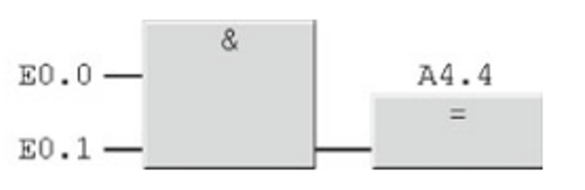
\includegraphics[width=\textwidth]{images/UndGatter.png}
    \caption{\textbf{UND-Gatter} [11]}
    \label{fig:undgatter}
  \end{subfigure}
  \hfill % Fügt flexiblen Abstand zwischen den Bildern ein
  \begin{subfigure}[b]{0.31\textwidth}
    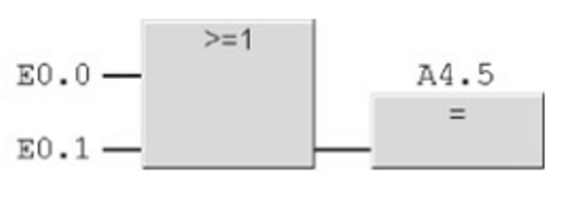
\includegraphics[width=\textwidth]{images/OderGatter.png}
    \caption{\textbf{ODER-Gatter} [11]}
    \label{fig:odergatter}
  \end{subfigure}
  \hfill
  \begin{subfigure}[b]{0.31\textwidth}
    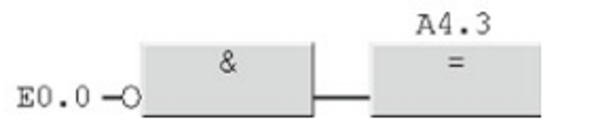
\includegraphics[width=\textwidth]{images/NotGatter.png}
    \caption{\textbf{NOT-Gatter} [11]}
    \label{fig:notgatter}
  \end{subfigure}
  
  \caption{Darstellung der logischen Grundfunktionen in FUP}
  \label{grundfufup}
\end{figure}


\textbf{Wichtige Funktionsbausteine in FUP}


\begin{figure}[htbp]
  \centering
  \begin{subfigure}[b]{0.49\textwidth}
    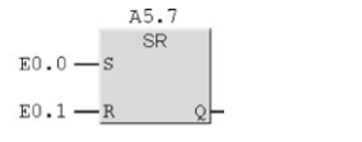
\includegraphics[width=\textwidth]{images/SRFlipFlop.png}
    \caption{\textbf{SR-FLIPFLOP} [11]}
    \label{fig:srflipflop}
  \end{subfigure}
  \hfill % Fügt flexiblen Abstand zwischen den Bildern ein
  \begin{subfigure}[b]{0.49\textwidth}
    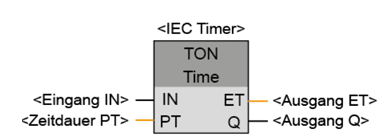
\includegraphics[width=\textwidth]{images/TON.png}
    \caption{\textbf{Einschaltverzögerung (TON)} [11]}
    \label{fig:ton}
  \end{subfigure}
  
  \caption{ Darstellung wichtiger Funktionsbausteine in FUP}
  \label{wichfunkbaust}
\end{figure}


In den obigen Abbildungen sind die wichtigsten Grundfunktionen und Funktionsbau
steine in \textbf{FUP} dargestellt. Mit diesen können diverse Abläufe realisiert werden, wie
beispielsweise einfache Förderbandsteuerungen. Komplexe, lange Abläufe sind jedoch
sehr aufwendig zu realisieren. Für eine SPS ist es daher gebräuchlich, hierfür auf
\textbf{ST/SCL} auszuweichen. In FUP können ebenfalls mathematische Operationen durch
geführt werden. Für Berechnungen existieren spezielle Bausteine. Allerdings ist es
schwierig, längere Rechenvorgänge übersichtlich darzustellen, da die Struktur schnell
unübersichtlich wird. Aus diesem Grund werden für sämtliche mathematische Opera
tionen häufig Berechnungen in \textbf{ST/SCL} durchgeführt. Beim vorliegenden Modell, dem
Hochregallager, wurde beispielsweise die Positionsermittlung der Lagerplätze für das
automatisierte Einlagern im vergangenen Studienprojekt in \textbf{SCL} realisiert.

\textbf{Grundlegende Anweisungen in SCL}


Im vorliegenden Projekt wird mit einer Siemens SPS gearbeitet. Somit ist SCL (Structu
red Control Language) der Standard im Bereich textbasierte Programmierung.
Hierbei gibt es einige konkrete Anweisungen, welche eine übersichtliche Programmie
rung gewährleisten.

Zu diesen zählen:

    \begin{itemize}
        \item \textbf{Zuweisungen:} Variable := Wert; Beispiel: Motor\_Start := TRUE;
        
        \item \textbf{Bedingte Anweisungen (IF-Strukturen):} IF Sensor = TRUE THEN Motor := TRUE; END\_IF;
        
        \item \textbf{Mehrzweigige Bedingungen (IF-ELSIF-ELSE):} IF Temp > 50 THEN Alarm := TRUE; ELSIF Temp > 30 THEN Warning := TRUE; ELSE Alarm := FALSE; END\_IF;
        
        \item \textbf{Schleifenstrukturen:} FOR i := 1 TO 5 DO Count := Count + 1; END\_FOR
        
        \item \textbf{Vergleiche und logische Operatoren:} AND, OR, NOT, >, <, =, >=, <=
        
    \end{itemize}

Diese Anweisungen ermöglichen selbst komplexe Programme zu realisieren. Es können
mathematische Berechnungen deutlich einfacher durchgeführt werden als beispielsweise in der Programmiersprache \textbf{FUP}.


\textbf{Vergleich SCL- FUP}


Die Programmiersprachen \textbf{FUP} und \textbf{SCL} werden beide für die Programmierung spei
cherprogrammierbarer Steuerungen verwendet.

Da \textbf{SCL} eine Siemens-eigene Sprache ist, konzentriert sich dieser Vergleich ausschließlich auf \textbf{STEP 7}.
Wie bereits erwähnt, ermöglicht \textbf{FUP} eine einfache blockbasierte Programmierung.
\textbf{FUP} eignet sich besonders für einfache Anwendungen, wie beispielsweise die Ansteue
rung von Drehstrommotoren. Auch für einfache Schrittketten ist \textbf{FUP} gut geeignet.
Mit zunehmender Programmkomplexität leidet jedoch die Übersichtlichkeit, was zu einer
erhöhten Fehleranfälligkeit führen kann.
Um diese Probleme zu vermeiden, wird in großen Produktionsanlagen mit komplexen Abläufen überwiegend textbasiert, also in \textbf{SCL}, programmiert. Die folgenden Darstellungen vergleichen beide Sprachen und verdeutlichen ihre Unterschiede. Dargestellt ist
eine einfache Förderbandsteuerung in \textbf{FUP} und \textbf{SCL} im TIA Portal.



\begin{figure}[htbp]
  \centering
  \begin{subfigure}[b]{0.49\textwidth}
    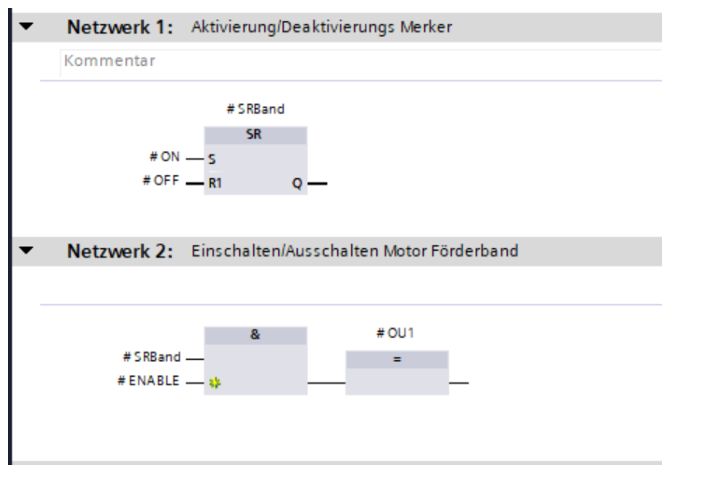
\includegraphics[width=\textwidth]{images/FBSteuerungFoerderband.png}
    \caption{Funktionsbaustein zur Steuerung des Förderbands}
    \label{fig:fbsteuerungfoeba}
  \end{subfigure}
  \hfill % Fügt flexiblen Abstand zwischen den Bildern ein
  \begin{subfigure}[b]{0.49\textwidth}
    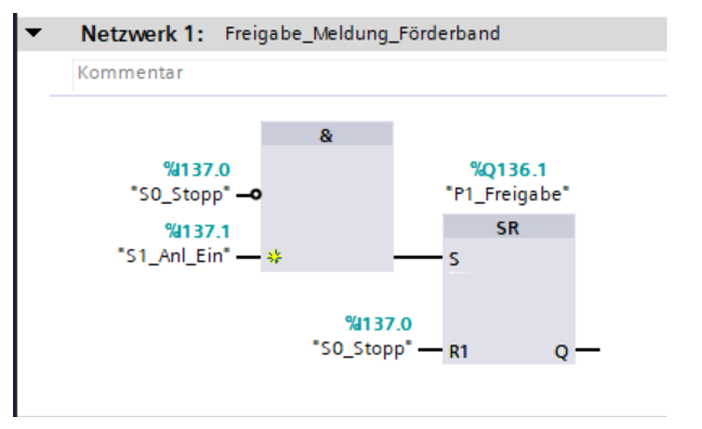
\includegraphics[width=\textwidth]{images/FreigabeImOB.png}
    \caption{Freigabe im Haupt-OB}
    \label{fig:freigahauptob}
  \end{subfigure}
  
  \caption{Realisierung der Förderbandsteuerung in FUP}
  \label{foebafup}
\end{figure}


\begin{figure}[htbp]
  \centering
  
  % Linker Codeblock (a)
  \begin{subfigure}[t]{0.45\textwidth}
\begin{lstlisting}
IF #OFF THEN
    #SR_Band := FALSE;
ELSIF #ON THEN
    #SR_Band := TRUE;
END_IF;

#OU1 := #SR_Band AND #ENABLE;

\end{lstlisting}
    \caption{SCL-Code des Förderband-Bausteins}
    \label{fig:scl_baustein}
  \end{subfigure}
  \hfill
  % Rechter Codeblock (b)
  \begin{subfigure}[t]{0.50\textwidth}
\begin{lstlisting}
IF NOT "S0_Stop" AND "S1_Anl_Ein" THEN
    "P1_Freigabe" := TRUE;
ELSIF "S0_Stop" THEN
    "P1_Freigabe" := FALSE;
END_IF;

"Foerderband"(
  OFF    := "B2_vorne",
  ON     := "B1_hinten",
  ENABLE := "P1_Freigabe",
  OU1    => "Q1_Band");

\end{lstlisting}
    \caption{Aufruf des Förderband-Bausteins im Hauptprogramm}
    \label{fig:scl_aufruf}
  \end{subfigure}

  \caption{Realisierung des Förderbandprogramms in \textbf{SCL}}
  \label{foerderband_scl}
\end{figure}

\clearpage

Anhand des Beispiels mit den Abbildungen \ref{foebafup} und \ref{foerderband_scl} wird deutlich, dass \textbf{FUP} auf den ersten Blick leichter
verständlich wirkt, da es sich um die grafische Verschaltung logischer Funktionen
handelt.
Auf den zweiten Blick zeigt sich jedoch, dass der Programmieraufwand deutlich höher
ist als in \textbf{SCL}. In \textbf{SCL} kann dieselbe Funktionalität mit wenigen, klar strukturierten
Codezeilen realisiert werden, ohne das Programm mit zusätzlichen Netzwerken zu
überladen.
Zusammenfassend lässt sich festhalten, dass sowohl \textbf{FUP} als auch \textbf{SCL} ihre jeweiligen
Vor- und Nachteile besitzen. Je nach Anwendung und Komplexität des Prozesses fällt
die Entscheidung für die eine oder die andere Programmiersprache

\subsubsection{Industrielle Bussysteme}
In der Automatisierung sind Kommunikationsprotokolle entscheidend für die Vernetzung
einzelner Systeme. Die Funktionalität einer automatisierten Anlage basiert auf der
erfolgreichen Kommunikation der einzelnen Komponenten.
Bussysteme in der Automatisierungstechnik
Ein großer Bestandteil im Bereich der Kommunikation zwischen verschiedenen Teilneh
mern bilden sogenannte Bussysteme.
Sie kommen zum Einsatz, wenn eine Steuerung mit den Sensoren bzw. Aktoren eines
Systems effizient kommunizieren soll. Die Steuerung kann z.B. eine \textbf{SPS} oder ein
\textbf{Mikrocontroller} sein.
Früher wurden Signale hauptsächlich über Hartverdrahtung übertragen. Diese Methode
war zwar zuverlässig, jedoch sehr aufwändig zu implementieren und mit hohem Material
und Zeitaufwand verbunden.
Deshalb wurden die bereits erwähnten Bussysteme eingeführt. Mit deren Hilfe ist es
möglich, mit geringem Verdrahtungsaufwand mit mehreren Teilnehmern innerhalb eines
Systems zu kommunizieren.
Ein Bussystem besteht grundsätzlich aus einer Leitung, über die mehrere Teilnehmer
angesprochen werden können. Die Topologie ist hierbei vielfältig. Es gibt sogenannte
\textbf{Stern-}, \textbf{Linien-} oder auch \textbf{Ring-Topologien}.


    \begin{figure}[H]
        \centering
        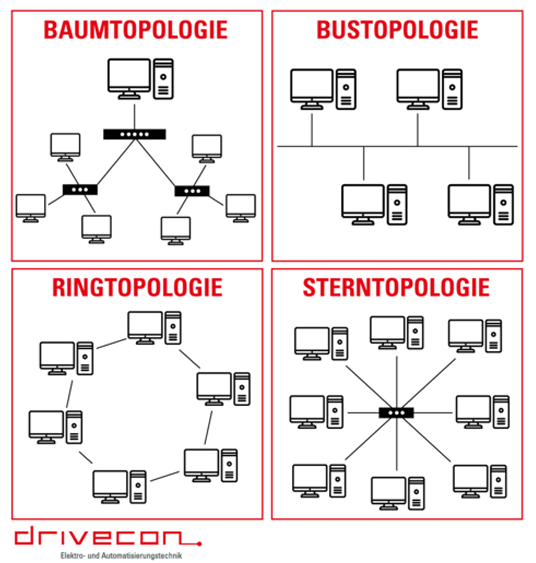
\includegraphics[width=\textwidth/2]{images/BusTopologien.png}
        \caption{Gängige Bus- Topologien; Quelle [6]}
        \label{bustopologien}
    \end{figure}


Die am häufigsten angewandte Methode ist die Kommunikation über eine \textbf{Linientopologie}.
Hierbei werden mehrere Teilnehmer über einzelne Abzweige nacheinander angesteuert.
Bussysteme können auf den verschiedensten Ebenen der Automatisierungspyramide[5]
zum Einsatz kommen. Der Haupteinsatz erfolgt jedoch auf der Feld- und Steuerungs
ebene.
Weiterhin gibt es verschiedene Arten von Bussystemen, die sich in ihrer Struktur, Ge
schwindigkeit und Übertragungsart unterscheiden. Die am häufigsten verwendeten sind
im Folgenden aufgelistet:

\begin{itemize}
    \item Feldbus-basierte Kommunikationssysteme (z.B. \textbf{Profibus})
    
    \item Ethernet-basierte Kommunikationssysteme (z.B. \textbf{PROFINET})
    
    \item Punkt-zu-Punkt-Systeme (z.B. \textbf{IO-Link})
\end{itemize}


Im Folgenden eine kurze Gegenüberstellung der einzelnen Protokolle:


\begin{center}
    % Erzeugt eine normale Tabellenbeschriftung ohne \begin{table}

    \begin{tabular}{|p{4cm}|p{3.5cm}|p{3.5cm}|p{3.5cm}|}
        \hline
            \textbf{Kriterium} & \textbf{IO-Link} &\textbf{PROFINET} &\textbf{PROFIBUS}\\
            \hline
            \textbf{Kommunikations- prinzip} & Punkt-zu-Punkt (PTP) & Ethernet-basiert& Feldbus-basiert \\
            \hline
            \textbf{Topologie}& Baum & Linie, Stern, Ring & Linie, Baum\\
            \hline
            \textbf{Kommunikations- rate} &4,8/ 38,4/ 230,4k Baud & bis 100Mbit/s & bis 12Mbit/s\\
            \hline
            \textbf{Typische Anwendung} & Sensorik, Aktorik, Handhabungstechnik & Steuerung, Kommunikation, Anlagenvernetzung& Maschinensteuer., Antriebsregelung\\
            \hline
    \end{tabular}

    \captionof{table}{Vergleich der Kommunikationssysteme IO-Link, PROFINET und PROFIBUS; Quellen: [5][15][14]}
    \label{tab:vergleichIOlinkprofinetprofibus}
\end{center}

\subsubsection{IO-Link}
IO-Link ist ein Kommunikationssystem, welches der Anbindung intelligenter Sensoren
und Aktoren dient.
Es wurde entwickelt, um die Lücke zwischen Feldbussen und Industrial-Ethernet
Systemen zu schließen. Der Standard ist in der Norm IEC 61131-9 definiert. IO-Link
wird häufig in Fabrikautomatisierungsanlagen eingesetzt.

\textbf{Aufbau und Funktionsweise von IO-Link}
IO-Link ist ein Kommunikationssystem, das nach dem \textbf{Point-to-Point} (PTP)-Prinzip
arbeitet. Das bedeutet, es werden mehrere Teilnehmer Punkt zu Punkt angesteuert.

Der \textbf{IO-Link-Master} ist hierbei mit den \textbf{IO-Link-Devices} PTP-verbunden. Dieser stellt
die Schnittstelle zwischen der Steuerung (\textbf{SPS}) und der Sensor-/Aktor-Ebene dar.


    \begin{figure}[H]
        \centering
        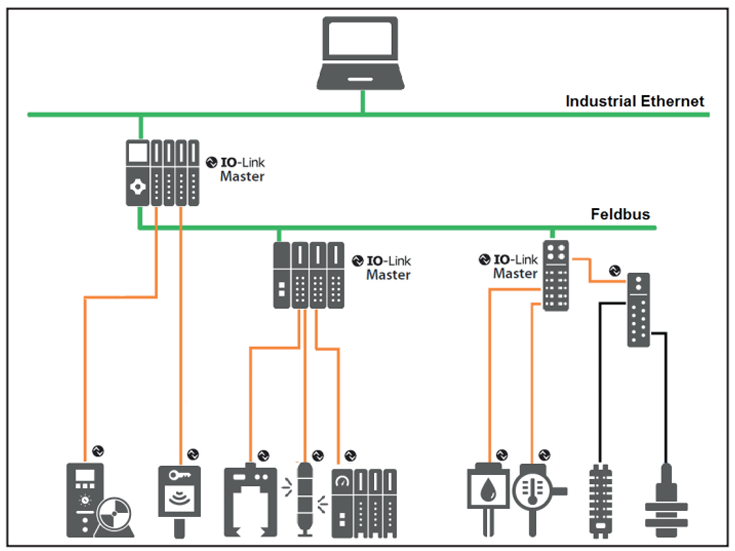
\includegraphics[width=350px]{images/IOLinkArchitektur.png}
        \caption{Architektur IO-Link; Quelle [5]}
        \label{}
    \end{figure}



Das System arbeitet \textbf{bidirektional}[5]. 
Das bedeutet, der IO-Link-Master kann sowohl
Prozessdaten empfangen als auch neue Parameter an die Devices senden (z.B. \textbf{RFID}).
Die Verbindung erfolgt über dreipolige Standardleitungen2.10. Dadurch lässt sich IO
Link problemlos in das Gesamtsystem integrieren. Eine separate Busverkabelung ist
nicht notwendig[2].


    \begin{figure}[H]
        \centering
        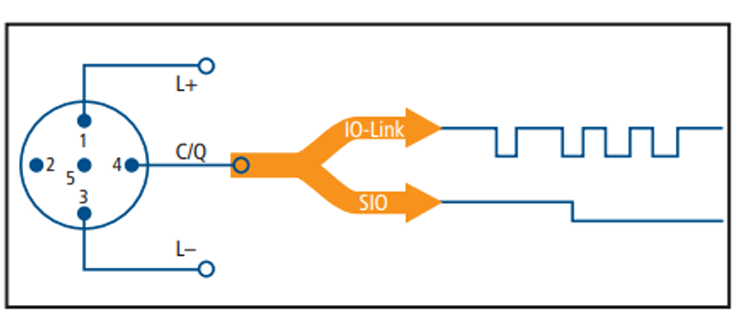
\includegraphics[width=500px]{images/IOLinkAnschluss.png}
        \caption{Anschlussbelegung IO-Link; Quelle [5]}
        \label{iolinkanschluss}
    \end{figure}

Der IO-Link-Master2.11 kann über ein übergeordnetes Bussystem (z.B. \textbf{Profibus},
\textbf{PROFINET}) mit der SPS kommunizieren[14].


    \begin{figure}[H]
        \centering
        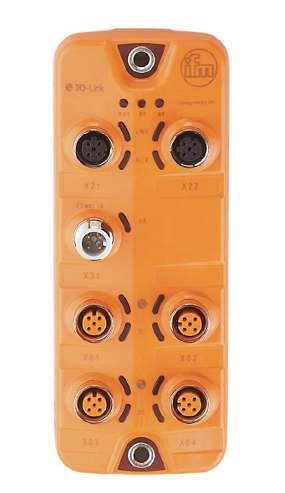
\includegraphics[width=\textwidth/3]{images/IOLinkMaster.png}
        \caption{Master IO-Link; Quelle [9]}
        \label{iolinkmaster}
    \end{figure}

\textbf{Kommunikation und Datenaustausch} Die Kommunikation über IO-Link erfolgt seriell. Hierbei wird mit festen Baudraten von 4,8kBaud, 38,4kBaud oder 230,4kBaud übertragen.
Die Datenkommunikation gliedert sich in drei Hauptarten[5]:

\begin{itemize}
    \item \textbf{Prozessdaten}:
    Diese werden zyklisch zwischen Master und Device ausgetauscht. Sie enthalten
    z. B. Messwerte von Sensoren oder Schaltzustände von Aktoren.
    \item \textbf{Servicedaten (Parameterdaten)}:
    Sie werden azyklisch übertragen und dienen zur Parametrierung oder Konfigu
    ration der Geräte. So können beispielsweise Schaltpunkte, Messbereiche oder
    Filterzeiten direkt über die Steuerung angepasst werden.
    \item \textbf{Ereignisdaten}:
    Hierbei handelt es sich um Status- oder Fehlermeldungen, die das Device bei
    bestimmten Zuständen (z. B. Übertemperatur, Kabelbruch oder Spannungsfehler)
    an den Master sendet.
\end{itemize}

Durch diese Aufteilung ist eine gezielte Überwachung, Diagnose bei Fehlern und
Konfiguration der einzelnen Module möglich. Eine Prozessunterbrechung ist hierfür
nicht notwendig.

Auf Protokollebene wird zwischen drei Schichten unterschieden[5]:


\begin{itemize}
    \item \textbf{Physikalische Schicht}: Definiert die elektrische Verbindung über die dreipolige Leitung.

    \item \textbf{Datenverbindungsschicht}: Regelt das Telegrammformat und die Fehlererkennung.

    \item \textbf{Applikationsschicht}: Beschreibt den Austausch von Prozess-, Service- und Ereignisdaten.
\end{itemize}


\textbf{Komponenten eines IO-Link-Systems}


Ein vollständiges IO-Link-System besteht in der Regel aus folgenden Komponenten[5]:

\begin{itemize}
    \item \textbf{IO-Link-Master}: Er verwaltet die Kommunikation zu den einzelnen IO-Link-Devices und bildet die Schnittstelle zur übergeordneten Steuerung. Je nach Ausführung kann der Master als Schaltschrankmodul oder als Feldmodul ausgeführt sein. Letzteres wird direkt in der Anlage montiert, wodurch sich Installationsaufwand und Verkabelungslänge reduzieren.
    
    \item \textbf{IO-Link-Devices}: Hierbei handelt es sich um Sensoren, Aktoren oder andere Feldgeräte, die über IO-Link kommunizieren. Typische Beispiele sind Drucksensoren, Wegmesssysteme, Ventilinseln, RFID-Leseeinheiten oder Smart Lights. Jedes Device verfügt über eine IODD-Datei (IO Device Description), in der alle Geräteparameter, Kom
    munikationsdaten und Diagnosemöglichkeiten beschrieben sind. Diese Datei wird
    im Engineering-Tool der Steuerung verwendet, um das Gerät automatisch zu
    erkennen und korrekt zu parametrieren.

    \item \textbf{Verkabelung}:
    IO-Link nutzt standardisierte, ungeschirmte Leitungen mit M12- oder M8-Steckverbindern.
    Die Kabellängen betragen typischerweise bis zu 20m zwischen Master und Device.
    Da das Signal digital übertragen wird, ist die Verbindung unempfindlich gegenüber
    elektromagnetischen Störungen und Spannungsabfällen.
\end{itemize}

\textbf{Zusammenfassung}

Über IO-Link ist eine Kommunikation bis in die unterste Feldebene möglich. Analoge
Signale sind hierbei überflüssig, da die Schnittstelle standardisiert ist. Weiterhin lassen
sich Geräte identifizieren und parametrieren. Außerdem stehen umfassende Diagno
semöglichkeiten zur Verfügung.
Damit trägt IO-Link wesentlich zur Transparenz, Flexibilität und Wartungsfreundlich
keit moderner Automatisierungssysteme bei und bildet eine wichtige Grundlage für
Konzepte wie \textbf{Industrie 4.0}[5].


\subsubsection{Vorteile und Nutzen in der Praxis}
Der Einsatz von IO-Link in der Industrie bringt zahlreiche Vorteile mit sich. Es werden
technische Defizite von klassischen Bus- und Anschlusssystemen eliminiert. Neben der
Vereinfachung der Verdrahtung bietet das System eine hohe Flexibilität, verbesserte
Diagnosefähigkeiten sowie eine sehr gute digitale Kommunikation bis in die Feldebene
hinein.

Durch die genannten Punkte wird nicht nur die Leistungsfähigkeit der Anlage gesteigert,
sondern auch die Wirtschaftlichkeit und Nachhaltigkeit in einer Produktion verbessert.


\textbf{Technische Vorteile}
Ein zentraler technischer Vorteil von IO-Link besteht in der vollständig digitalen Signal
übertragung zwischen dem IO-Link-Master und den angeschlossenen Devices. Dadurch
entfallen typische Nachteile analoger Schnittstellen wie Messfehler durch Spannungsab
fall, Rauschen oder Kalibrierungsabweichungen. Jeder über IO-Link verbundene Sensor
oder Aktor überträgt exakte Prozessdaten in digitaler Form, wodurch die Messqualität
und Zuverlässigkeit deutlich erhöht werden.
Ein weiterer Vorteil ist die sogenannte bidirektionale Kommunikation. Hierbei ist es
möglich, dass der IO-Link-Master Daten empfangen kann, sowie in der Lage ist, die
Parameter der Sensoren oder Aktoren zu beschreiben.
Darüber hinaus bietet IO-Link standardisierte Schnittstellen und Datenstrukturen, die
herstellerübergreifend kompatibel sind. Jedes Gerät wird anhand seiner IODD-Datei (IO
Device Description) automatisch erkannt, was die Integration in bestehende Systeme
erheblich vereinfacht[5]. Diese Einheitlichkeit führt zu einer hohen Austauschbarkeit der
Komponenten, ohne dass Änderungen in der SPS-Software oder in der Verdrahtung
notwendig sind.


\textbf{Weitere Vorteile}



Durch den verringerten Verdrahtungsaufwand können erhebliche Kosten eingespart
werden. Diese können an anderer Stelle effizienter eingesetzt werden.
Da ein IO-Link-Master in der Lage ist, sowohl klassische als auch digitale Signale zu
verarbeiten, entfallen zusätzliche Baugruppen zur Verarbeitung bestimmter Signalarten.
Diese Punkte führen zu einer Erhöhung bzw. Verbesserung der Wirtschaftlichkeit.
Dadurch kann nachhaltiger und effektiver gearbeitet werden.


\textbf{Erweiterte Diagnosemöglichkeiten}


Eine besondere Eigenschaft von IO-Link liegt in den umfassenden Diagnosemöglichkeiten, die dem Anwender zur Verfügung stehen. Jedes Device ist in der Lage, sich selbst
zu diagnostizieren und die entsprechenden Informationen an den \textbf{IO-Link-Master} zu
übermitteln.
Somit werden Fehler wie Kabelbruch, Kurzschluss oder Unterspannung sofort an die
Steuerung gemeldet. Dadurch ist ein schnelles und effektives Trouble Monitoring ge
geben. Dies führt dazu, dass langfristig Fehlerquellen und Anfälligkeiten in Systemen
erkannt und gezielt beseitigt werden können.


\textbf{Praxisbeispiel}


In der industriellen Praxis findet IO-Link zunehmend Anwendung bei intelligenten Sen
soren und Aktoren, etwa in Montage- und Prüfprozessen oder bei der Handhabungs
technik.
Ein typisches Beispiel ist die Integration eines IO-Link-Füllstandssensors oder Druck
sensors in ein SPS-System. Die Messwerte werden dabei digital und störungsfrei
übertragen, während gleichzeitig Geräteparameter über die Steuerung angepasst wer
den können, etwa der Schaltpunkt oder der Messbereich[5].



\textbf{Zusammenfassung}


IO-Link vereint einfache Installation mit intelligenter Kommunikation. Die Technologie
schafft eine durchgängige Datenbasis von der Feldebene bis zur Steuerung und ermög
licht so eine effiziente, flexible und zukunftssichere Automatisierung.
Durch die Kombination aus digitaler Signalübertragung, erweiterter Diagnose und au
tomatischer Parametrierung wird IO-Link zu einem zentralen Bestandteil moderner
Industrie-4.0-Architekturen.


\subsubsection{Sicherheit in der Automatisierung}
m Kontext der Automatisierung von technischen Anlagen ist die Sicherheit der größte
und wichtigste Aspekt [4].
Beim Betreiben eines Systems muss vollständig ausgeschlossen sein, dass keine
Gefahr für Menschen, von der Anlage, ausgeht. Das bedeutet, bei Planung der Anlage,
steht die Sicherheit im Fokus.
Speziell in der Produktion bzw. in der Logistik sind sicherheitstechnische Aspekte enorm
wichtig.
Bei automatisierten Prozessen wie z.B. das Verfahren eines Hochregallagers, können
Gefahren durch Implementierung von Sicherheitslogiken ausgeschlossen werden.
Das Ziel ist immer Gefährdungen bzw. Verletzungen von Menschen zu verhindern.


\textbf{Einordnung in den Kontext der funktionalen Sicherheit}

Um die Sicherheitsprinzipien besser zu verstehen, ist es wichtig, die einzelnen Aspekte
der Sicherheitsthematik im Gesamtkontext einzuordnen.
In diesem Zusammenhang spielt der Bereich der funktionalen Sicherheit eine entschei
dende Rolle.
Hierunter versteht man den Teil einer Maschine, der von den korrekt funktionierenden
Steuerungs- und Sicherheitskomponenten abhängt. Sie sorgt dafür, dass bei kritischen
Situationen ein sicherer Zustand der Anlage erreicht wird. Ein Beispiel hierfür wäre das
direkte Abschalten eines Motors[10].
Damit sicherheitsbezogene Steuerungssysteme zuverlässig arbeiten, müssen sie be
stimmte Anforderungen erfüllen, die in internationalen Normen festgelegt sind.


Einige dieser Vorschriften sind im Folgenden aufgelistet[10]:

\begin{itemize}
    \item \textbf{ENISO13849-1}: Beschreibt die sicherheitsrelevanten Teile einer Anlage, unter anderem den \textbf{PL} (Performance Level).
    \item \textbf{IEC 61508}: Behandelt die funktionale Sicherheit elektrischer, elektronischer und programmierbarer Steuerungssysteme. Basiert auf dem \textbf{SIL} (Safety Integrity Level).
    \item \textbf{EN61496}: Sicherheit von Maschinen– Berührungslos wirkende Schutzeinrichtungen (BWS), beispielsweise Lichtschranken oder Lichtvorhänge.
\end{itemize}

Die genannten Normen zeigen ebenfalls die Bedeutung der Sicherheit im Anlagenbau
für den Gesetzgeber. Falls es zu Verstößen kommen sollte, führt dies zu Konsequenzen
für den Arbeitgeber.
Das ist der Grund dafür, dass Unternehmen sehr genau auf die Einhaltung dieser
Vorschriften achten.
Für die genannten Normen gibt es dementsprechende Geräte, welche beispielsweise
im Fehlerfall (Fehlerstrom) abschalten sollen (FI-Schutzschalter).
Die Auswahl der Sicherheitskomponenten erfolgt auf Basis einer sogenannten \textbf{Risiko
beurteilung}. Diese ermittelt die potenziellen Gefahren und legt das \textbf{Performance Level}
bzw. den \textbf{SIL} fest. In der Praxis werden Sicherheitsfunktionen häufig mit einem \textbf{PL d}
oder \textbf{SIL 2} realisiert, da diese ein gutes Verhältnis zwischen Aufwand und Sicherheit
bieten.


Eine zentrale Rolle innerhalb dieser sicherheitsrelevanten Systeme spielt die \textbf{Sensorik}.
Sie dient als Grundlage zur Erfassung von Zuständen und Bewegungen innerhalb einer
Anlage und bildet somit die Basis für jede Sicherheitsfunktion.
Besonders in automatisierten Prozessen ist es wichtig, dass Gefahrenzonen zuverlässig
überwacht werden, ohne den Produktionsablauf zu beeinträchtigen.


Hier kommen berührungslos wirkende Schutzeinrichtungen zum Einsatz, wie beispiels
weise \textbf{Lichtschranken} oder \textbf{Lichtvorhänge}. Diese ermöglichen eine sichere und
zugleich flexible Absicherung von Arbeitsbereichen, an denen Mensch und Maschine
aufeinandertreffen.
Lichtschranken zählen zu den am weitesten verbreiteten Sicherheitseinrichtungen in
der Industrie und werden unter anderem bei Robotersystemen, Förderanlagen oder
automatisierten Handhabungsstationen verwendet.
Im folgenden Abschnitt wird die Funktionsweise, der Aufbau sowie der Einsatz von
Lichtschranken in sicherheitsrelevanten Anwendungen näher erläutert.

\subsubsection{Lichtschranken in sicherheitsrelevanten Anlagen}
Die Lichtschranke ist eine der wichtigsten Sicherheitseinrichtungen in der Fertigung und
Logistik.
Sie verhindert das unbefugte Eingreifen in laufende Prozesse, sodass mögliche Gefah
ren für Personen zuverlässig ausgeschlossen werden können.
Viele Hersteller bieten ihre Bauteile frei konfigurierbar an. Dadurch ist es möglich,
die Betriebsmodi und Parameter individuell an die jeweilige Anwendung anzupassen,
beispielsweise bei der Absicherung von Hochregallagern oder automatisierten Förder
anlagen.
Lichtschranken kommen in sicherheitsrelevanten Anlagen überall dort zum Einsatz, wo
Gefahrenbereiche zuverlässig überwacht werden müssen, ohne dass mechanische
Barrieren den Prozessfluss behindern.


\textbf{Funktionalität einer Lichtschranke}


Bei einer Lichtschranke handelt es sich um eine berührungslos wirkende Schutzeinrichtung, die mit einem oder mehreren Lichtstrahlen arbeitet. Diese Lichtstrahlen bilden
eine optische Barriere, die bei Unterbrechung ein Signal auslöst.
Eine Lichtschranke besteht grundsätzlich aus zwei Modulen: einem \textbf{Sender} und einem
\textbf{Empfänger}. Der Sender erzeugt ein Lichtsignal, das vom Empfänger erfasst wird. 

Wird
der Lichtstrahl unterbrochen, erkennt die Auswerteelektronik diesen Zustand und leitet
eine vordefinierte Sicherheitsreaktion ein, beispielsweise das Abschalten eines Antriebs oder das Anhalten eines Roboters.
Die am häufigsten verwendeten Lichtschrankentypen sind die \textbf{Reflexionslichtschranke}
und die \textbf{Infrarotlichtschranke}[3].
Bei einer \textbf{Reflexionslichtschranke} befinden sich Sender und Empfänger im selben
Gehäuse. Das ausgesendete Lichtsignal wird über einen Reflektor zurückgeworfen und
von der Empfangseinheit detektiert. Wird der Lichtstrahl durch ein Objekt unterbrochen,
bleibt das Signal aus und die Sicherheitsfunktion wird aktiviert.

Die im Projekt verwendete Variante ist eine \textbf{Infrarotlichtschranke}. Diese arbeitet mit
unsichtbarem Infrarotlicht, das unempfindlich gegenüber Umgebungslicht und Staub ist.

    \begin{figure}[H]
        \centering
        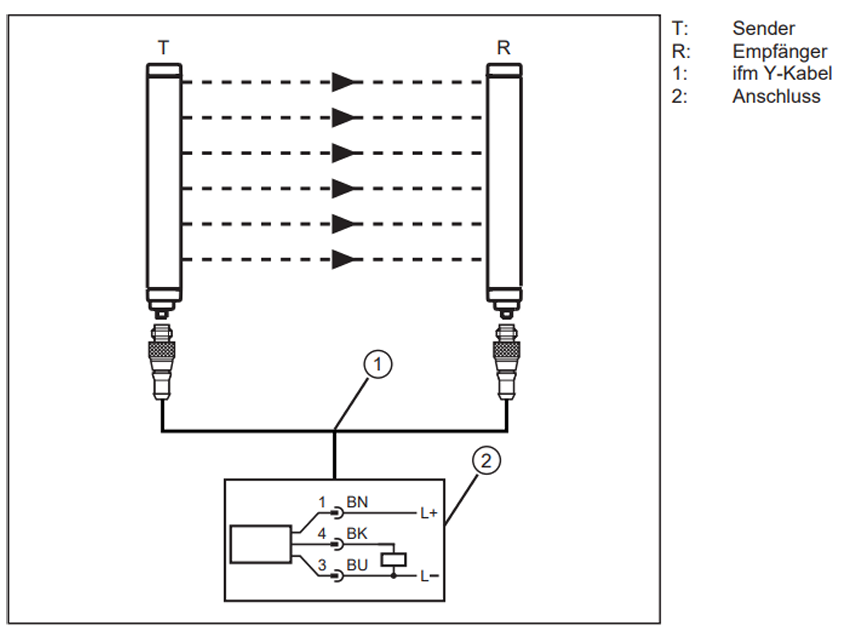
\includegraphics[width=350px]{images/SchematischeDarstellungIFMLichtgatter.png}
        \caption{Schematische Darstellung des IFM Lichtgatters[7]}
        \label{ifmlichtgatter}
    \end{figure}

Hierbei wird ein kontinuierlicher Infrarotstrahl vom Sender ausgesendet, der vom Empfänger registriert wird. Wird der Strahl unterbrochen, erkennt die Steuerung dies sofort
als Störung oder Eingriff und löst eine Sicherheitsreaktion aus 2.12.
Durch die hohe Reichweite und Störsicherheit eignet sich die Infrarotlichtschranke
besonders für industrielle Umgebungen, in denen eine präzise und zuverlässige Objek
terkennung gefordert ist.
Häufig variiert die Bezeichnung solcher Systeme. Viele Hersteller verwenden dafür auch
den Begriff \textbf{Lichtgitter} oder \textbf{Lichtvorhang}.
So auch der Hersteller \textbf{ifm}, der das im Projekt verwendete Produkt bereitstellt [8]. 

Diese
Systeme sind modular aufgebaut und lassen sich über verschiedene Schnittstellen
beispielsweise IO-Link direkt in eine Steuerung integrieren


    \newpage
    \section{Implementierung eines Lichtgatters in das Gesamtkonzept}
%%%%%%%%%%%%%%%%%%%%%%%%%%%%%%%%%%%%%%%%%%%%%%%%%%%%%%%%%%%%%%%%%%%%%%%%%%%%%%%%%%%%%%%%%%%%%%%%%%%%%%%%%%%%%%%%%%%%%%%%

Im aktuellen Ist-Zustand des Hochregallagers fehlt die vollständige Implementierung
der Sicherheitslogik.
Lediglich der Not-Aus-Schalter ist hardwareseitig verdrahtet und schaltet bei Betätigung
die Zuleitung ab. Es existiert jedoch keine automatische Abschaltung im Gefahrenfall.
Die Logik des Ein- und Auslagerns ist somit nicht gefahrenfrei. Sobald ein Eingriff in den
Prozess erfolgt, kann dieser im aktuellen Zustand nicht automatisch gestoppt werden.
Da das Miniaturmodell eine reale Situation in der Logistik abbilden soll, stellt dieser
Punkt ein erhebliches Defizit dar.
Es gibt verschiedene Möglichkeiten, um diesen Nachteil zu beheben. Die naheliegendste
Option ist die Implementierung einer Lichtgatter-Funktion, um den Gefahrenbereich
zuverlässig zu überwachen und den Betrieb im Störfall sicher zu unterbrechen. Durch
ein vorheriges Projekt wurde bereits, ein Modell der Firma IFM[8], installiert.

\subsection{Zielsetzung der Implementierung}
Die Studienarbeiten der vergangenen Jahre haben das Hochregallager in einen Zustand
gebracht, der wichtige Funktionen wie Ein- und Auslagern abbildet.
Jedoch wurden hierbei, fälschlicherweise, die notwendigen Sicherheitsaspekte völlig
außer Acht gelassen.
In einer realen Umgebung, beispielsweise in Materiallagern mit Hochregalsystemen
großer Industrieunternehmen, wäre eine solche Vorgehensweise undenkbar.
Es muss jederzeit gewährleistet sein, dass Gefahren so gut wie möglich unter Kontrolle
gehalten werden. Das bedeutet, im Fehlerfall muss jede gefährliche Bewegung sicher
abgeschaltet werden.
Dies stellt die zentrale Zielsetzung der Implementierung dar. In jedem Betriebsmodus
muss sichergestellt sein, dass bei Erkennung einer Gefahr automatisch abgeschaltet
wird.
Dabei ist jedoch zu berücksichtigen, dass der Kolben des Zylinders, welcher die Mate
rialien einlagert, kein Abschaltsignal auslösen darf. Dieser fährt nämlich unmittelbar in
den Gatterbereich der Lichtschranke ein.
Somit ist zunächst eine umfassende Analyse des Ist-Zustands sowie der verschiedenen
Prozesswerte des Lichtgatters erforderlich.
Erst im Anschluss kann die Implementierung der Sicherheitslogik erfolgen

\subsection{Analyse der Paramerierung des Lichtgatters}
Die Konfiguration des Lichtgatters ist entscheidend für die richtige Funktionsweise. Beim
Modell von IFM[8] gibt es mehrere Möglichkeiten zur Parametrierung.
Das Lichtgatter besitzt mehrere Lichtstrahlen, welche über einzelne Bits definiert sind.
Sobald sich ein Objekt im Gatter befindet, werden mehrere dieser Lichtstrahlen gleich
zeitig unterbrochen.
Der Sensor des vorliegenden Lichtgatters hat im sogenannten Detektionsmodus
(GTBO) den Wert 1. Das bedeutet, dass er schaltet, sobald ein Objekt die Strahlen
unterbricht.
Über IO-Link kann nun festgelegt werden, ab wie vielen unterbrochenen Strahlen der
Sensor ein Schaltsignal ausgeben soll

\subsubsection{Prozesswerte der Steuerung des Arbeitsverhaltens}
Zur Steuerung des Verhaltens bei einer Unterbrechung stehen verschiedene Prozess
werte zur Verfügung[7]:
• FBO(First Beam Occupied)
• LBO(Last Beam Occupied)
• CBO(Central Beam Occupied)
• NBO(Number of Beams Occupied)
• NCBO(Number of Consecutive Beams Occupied)
Im Betriebsmodus FBO schaltet der Sensor bereits beim ersten unterbrochenen Licht
strahl. Das bedeutet, Objekte, die im unteren Bereich des Lichtgatters liegen, werden
als erstes erfasst.
Im Modus LBO geschieht genau das Gegenteil: Es wird beim letzten Lichtstrahl ge
schaltet.
Dieser Modus wird beispielsweise bei Endlagenerkennungen oder beim Auslagern
verwendet– also immer dann, wenn das Austreten aus einem bestimmten Bereich
überwacht werden soll.
Der Modus CBO ist etwas komplexer: Hier wird der mittlere Lichtstrahl (bei mehreren
zusammenhängenden Strahlen) überwacht. Tritt ein Objekt in das Lichtgatter ein, wird
der zentrale Strahl als Referenzpunkt betrachtet. Bei mehreren Objekten wird immer
vom größeren Objekt ausgegangen, also von dem, das mehr Strahlen gleichzeitig
unterbricht– wie in Abbildung 3.13 zu sehen.
Automatisiertes Modell- Hochregallager
26
3 Implementierung eines Lichtgatters in das Gesamtkonzept
Anwendungsbeispiele sind z. B. Durchgänge oder Förderabschnitte, also überall dort,
wo Objekte mittig erfasst werden sollen (Referenzpunkt: Mitte).
Abbildung 3.13: Modus CBO; Quelle: [7]
Die letzten beiden Modi, NBO und NCBO, beschäftigen sich mit der konkreten Anzahl
der Lichtstrahlen, die unterbrochen werden.
Der Unterschied der beiden Modi liegt darin, dass NBO die Gesamtanzahl der unterbro
chenen Lichtstrahlen angibt, während NCBO die Anzahl der Strahlen beschreibt, die
aufeinanderfolgend unterbrochen werden.
Im Projekt wird der Modus NBO verwendet. Eine Abbildung soll die Funktionsweise
noch einmal verdeutlichen (siehe Abbildung 3.14)

\subsection{Komponentenübersicht und Systemaufbau}
FürdieUmsetzungderSicherheitsfunktionwurdeeinSystemaufbaurealisiert,derdie
LichtschrankedirektmiteinemIO-Link-MasterundderSPSverbindet.ImFolgenden
werdendieeingesetztenKomponentensowiederenZusammenspiel innerhalbdes
Gesamtsystemsbeschrieben.
Komponente Hersteller/Typ Funktion Schnittstelle
Lichtgitter / Licht
schranke
IFMOY5100(Infrarot) Erfassung von Objekten
undÜberwachungdesGe
fahrenbereichs
IO-Link
IO-LinkMaster IFMAL1100 Kommunikation zwischen
IO-Link-Devices und der
SPS
PROFINET /
IO-Link
SPS SiemensS7-1500 Steuerungdesgesamten
Systems,Verarbeitungder
Sensorsignale
PROFINET
Netzteil24VDC SiemensSITOP/ver
gleichbar
Versorgung von IO-Link
Master,Lichtschrankeund
SPS
24VDC
Aktorik(Zylinder/Mo
tor)
Festo(pneumatisch) Ausführungder Ein- und
Auslagerbewegung
Digitale Aus
gänge der
SPS
Tabelle4:ÜbersichtderverwendetenKomponentenimSystemaufbau
InTabelle4sinddieeinzelnenKomponentendesHochregallagersrundumdieLicht
schrankedargestellt.
Diesemüssenoptimalmiteinanderinteragieren,umdiegewünschteFunktionalitätsi
cherzustellen.
DieLichtschrankeistvomTypOY5100undstammtvomHerstellerIFM.Eshandeltsich
hierbeiumeinsteuerbaresLichtgitter,dasüberIO-LinkmitderSPSkommuniziert.

\subsubsection{Systemaufbau}
Die folgende Abbildung zeigt den strukturellen Aufbau des Gesamtsystems in verein
fachter Form.
SPS
(Siemens S7-1500)
Netzteil
24V DC
24V DC
PROFINET
IO-Link Master
(IFM AL1100)
IO-Link
Lichtgitter
(IFM OY5100)
Signal / Reaktion
Aktorik
(Zylinder / Motor)
Abbildung 3.15: Vertikaler Systemaufbau des Lichtgatter-Systems
Im Diagramm 3.15 ist der Aufbau der einzelnen Komponenten grafisch dargestellt. Der
IO-Link-Master dient hierbei als Schnittstelle zwischen SPS und Lichtgitter und steuert
die Kommunikation über das im TIA Portal implementierte Programm.
Im Fehlerfall werden gefährliche Bewegungen, die beispielsweise vom Zylinder oder
den Motoren der Linearachsen ausgehen, automatisch gestoppt.
Im folgenden Abschnitt wird die Implementierung dieser Sicherheitslogik in der SPS
detailliert erläutert

\subsection{Implementieren der Sicherheitslogik in die SPS}
Die Sicherheitslogik wird, wie bereits erwähnt, in eine Siemens S7-1500 SPS einpro
grammiert. Die Programmierung erfolgt mithilfe der Software TIA Portal.
Für die Umsetzung der Arbeit wurde das bestehende Programm des Jahrgangs TEA
22 als Grundlage verwendet. Zunächst wurde eine neue Program Organization Unit
(POU) mit der Bezeichnung Lichtschranke erstellt.
Im Anschluss erfolgte das Einbinden des Moduls OY5100 im Reiter Geräte und Netz
werke. Der Adressbereich (frei wählbar) wurde so konfiguriert, dass eine eindeutige
Zuordnung innerhalb des Projekts gewährleistet ist.
Abbildung 3.16: Einbindung der IFM-Lichtschranke OY5100 im TIA Portal
Die zugewiesenen Adressen werden für die verschiedenen Prozesswerte genutzt (siehe
Kapitel 3.2.1).
Als Vorbereitung auf die Programmierung wurde eine sogenannte Watchtable erstellt.
Diese dient dazu, die einzelnen Prozesswerte des Lichtgatters während der Laufzeit zu
überwachen und deren Verhalten zu analysieren.
Die Prozesswerte liegen im Format WORD (2 Byte) vor und bilden die Anzahl der
unterbrochenen Lichtstrahlen ab.
Nach einer Reihe von Tests wurde festgestellt, dass der Kolben des Zylinders im Ar
beitsbereich des Lichtgatters drei Strahlen gleichzeitig unterbricht. Hierfür erfolgte
ein gezieltes Verfahren der Lineareinheit über alle vier Ebenen des Hochregallagers.
So konnte überprüft werden, dass der Kolben in jeder Position konstant drei Strahlen
abdeckt.
Im weiteren Verlauf wurde diskutiert, welcher Prozesswert sich für die Sicherheitslogik
am besten eignet. Es zeigte sich, dass der Modus NBO (Number of Beams Occupied)
Automatisiertes Modell- Hochregallager
30
3 Implementierung eines Lichtgatters in das Gesamtkonzept
die Summe aller unterbrochenen Lichtstrahlen angibt (siehe Kapitel 3.2.1). Daher ist
dieser Prozesswert optimal geeignet, um eine zuverlässige Abschaltung über das Licht
gatter zu realisieren.
Nach der Diskussion wurde, für die Realisierung der Abfrage, ein neuer FB (Freigabe-Lichtschranke-FB24) aufgebaut in SCL. Im Diagramm 3.17 ist der Zusammenhang
zwischen den einzelnen Modi und der Freigabe dargestellt.
FB
Handbetrieb
Signalaustausch
FB24
Freigabe
Lichtschranke
Status / Freigabe
FB
Prozesssteuerung
(Ein-/Auslagerung)
Rückmeldung / Fehler
FB
Störungen
Abbildung 3.17: Einbindung des Bausteins FB24 Freigabe\_Lichtschranke in das
Gesamtsystem
Der Baustein FB24 Freigabe\_Lichtschranke ist ein zentraler Bestandteil der Sicher
heitsarchitektur.
Ohne ihn wäre ein sicheres Abschalten im Fehlerfall nicht möglich. Die Prozesssteue
rung wird durch die Freigabe in jedem Schritt überwacht.
Durch die Einbindung in den FB11 Strungen erfolgt eine Überwachung sämtlicher
Ausgänge über die Variable b\_Freigabe. Diese wird gesetzt, sobald keine Störungen
aktiv sind und die Freigabe durch das Lichtgitter gegeben ist.
Automatisiertes Modell- Hochregallager
31
3 Implementierung eines Lichtgatters in das Gesamtkonzept
Abbildung 3.18: Setzen der Variable b\_Freigabe in FB11 Strungen
Jene Variable in Abbildung 3.18 wurde bereits in vorherigen Projekten verwendet.
Sie wird im Block FB\_Ausgnge eingesetzt, als zusätzliche invertierte Rücksetzbedin
gung. Somit ist ein fehlerfreier Betriebsmodus der einzelnen Aktoren gewährleistet.


\subsubsection{Logische Abschaltbedienungen der Lichtschranke}

In Abbildung 3.19 ist der Ablauf der Sicherheitsabschaltung grafisch dargestellt. Sobald
der Prozesswert NBO größer als 3 ist, wird die Aktorik abgeschaltet. Das bedeutet,
dass eine sofortige Abschaltung erfolgt, sobald zusätzlich zum Zylinder eine Hand oder
ein anderes Objekt detektiert wird– also ein weiterer Lichtstrahl unterbrochen ist.


\subsection{Visualisierung auf dem HMI}
In diesem Kapitel wurde die Implementierung einer sicherheitsgerichteten Lichtschranke
in das bestehende Hochregallager-System beschrieben. Dabei erfolgte zunächst die
Analyse der Prozesswerte des IFM-Lichtgatters sowie die Auswahl des geeigneten
Betriebsmodus zur sicheren Erkennung von Objekten im Gefahrenbereich. Anschlie
ßend wurde der vollständige Systemaufbau erläutert und die Anbindung über den
IO-Link-Master an die Siemens-SPS umgesetzt. Die daraus resultierende Sicherheitslo
gik ermöglicht es, gefährliche Bewegungen im Fehlerfall automatisch zu stoppen und
so die funktionale Sicherheit des Systems zu gewährleisten.
Die Visualisierung der Sicherheitszustände erfolgt über den integrierten Störungsbau
stein des HMI-Panels, wodurch Unterbrechungen und Fehlermeldungen automatisch
angezeigt werden. Eine Erweiterung dieser Funktion um eine gezielte Anzeige des
Anlagenzustands (z.B. „Normalbetrieb“, „Sicherer Halt“) bietet zusätzliches Potenzial
zur Verbesserung der Bedienerfreundlichkeit und Systemtransparenz.
Damit ist die sicherheitstechnische Basis des Hochregallagers geschaffen, auf der im
folgenden Kapitel weitere Funktionen und Erweiterungen aufgebaut werden können


    \newpage
    \section{Implementierung eines Umlagerungsprozesses}
%%%%%%%%%%%%%%%%%%%%%%%%%%%%%%%%%%%%%%%%%%%%%%%%%%%%%%%%%%%%%%%%%%%%%%%%%%%%%%%%%%%%%%%%%%%%%%%%%%%%%%%%%%%%%%%%%%%%%%%%
\subsection{Definition "Umlagerung" im Kontext der Intralogistik}
In der Intralogistik bezeichnet eine Umlagerung die interne Verlagerung von Mate
rial oder Ladeeinheiten innerhalb eines Lagersystems, ohne dass ein Warenein
oder-ausgang erfolgt. Sie dient nicht der Erfüllung eines Kundenauftrags, sondern
der Optimierung der Lagerstruktur und der Betriebsabläufe. Typische Gründe für
Umlagerungen sind:
• Platzoptimierung: Zusammenführen von Teilpaletten oder das Freiräumen be
stimmter Stellplätze für neue Einlagerungen.
• Reduktion der Zykluszeiten: Lagerware, die weit weg von der Entnahmestelle
eingelagert wurde, wird in Totzeiten des Systems näher an die Entnahmestelle
umgelagert. Dies verkürzt die Zykluszeit bei späterer Anfrage der Ware.
• Strategische Positionierung: Umlagerung von Artikeln in Bereiche mit höherer
Zugriffshäufigkeit, um Kommissionierzeiten zu reduzieren.
• Qualitätssicherung: Verbringen von Waren in Quarantäne- oder Prüfzonen.
• Technische Anforderungen: Freihalten von Stellplätzen für Wartungsarbeiten
oder zur Vermeidung von Blockaden.
• Bestandskorrekturen: Anpassungen nach Inventuren oder bei fehlerhaften Bu
chungen.
Im Gegensatz zu Ein- und Auslagerungen, die externe Materialflüsse abbilden, ist die
Umlagerung ein rein interner Prozess.



\subsection{Prozessablauf der Umlagerung}
In diesem Kapitel wird der Funktionsablauf aus einer systemorientierten Perspekti
ve betrachtet. Ziel ist es, die Interaktion der beteiligten Komponenten sowie die
Abhängigkeiten zwischen mechanischen Bewegungen, Steuerungslogik und
Sicherheitsmechanismen darzustellen. Darüber hinaus werden die wesentlichen
Prozessschritte erläutert, die für einen störungsfreien Betrieb erforderlich sind. Die
Darstellung erfolgt unabhängig von der konkreten Programmierung, um eine klare
Trennung zwischen konzeptioneller Beschreibung und technischer Umsetzung zu
gewährleisten.
Automatisiertes Modell- Hochregallager
34
4 Implementierung eines Umlagerungsprozesses
Entwurf der Schrittkette für Umlagerungen
Die im Rahmen dieser Arbeit implementierte Umlagerungsfunktion basiert konzeptionell
auf den bereits vorhandenen Schrittketten für die Einlagerungs- und Auslagerungspro
zesse. Beide Abläufe bilden die Grundlage für die Umlagerung, da sie die wesentlichen
Bewegungs- und Steuerungslogiken enthalten, die für den sicheren Transport von Lade
einheiten erforderlich sind. Die Umlagerung kombiniert diese beiden Prozessketten in
einer strukturierten Sequenz: Zunächst wird die Ladeeinheit am Quellplatz aufgenom
men (analog zur Auslagerung), anschließend erfolgt die Verfahrbewegung zum Zielplatz
und die Ablage (analog zur Einlagerung).
Allerdings wurde für die Realisierung der Umlagerungsfunktion eine eigenständige
Schrittkette entwickelt. Dies war notwendig, da der Umlagerungsprozess im Vergleich
zu den bestehenden Abläufen zusätzliche Anforderungen stellt: Zum einen sind mehr
Schritte erforderlich, um die vollständige Sequenz von Aufnahme, Transport und Ablage
abzubilden. Zum anderen müssen an zwei Stellen Verzweigungen integriert werden,
um unterschiedliche Prozesspfade abhängig von den Betriebsbedingungen zu ermög
lichen. Durch die Erstellung einer eigenen Schrittkette wird sichergestellt, dass die
Logik klar strukturiert bleibt und die zusätzlichen Schritte sowie Verzweigungen ohne
Beeinträchtigung der bestehenden Programme umgesetzt werden können.
Automatisiertes Modell- Hochregallager
35
4 Implementierung eines Umlagerungsprozesses
Besonderheiten der Umlagerungsschrittkette
Die Umlagerungsschrittkette stellt eine Erweiterung der bestehenden Abläufe für Ein
lagerung und Auslagerung dar, basiert jedoch nicht ausschließlich auf deren Struktur.
Während die Grundlogik der Bewegungen übernommen wurde, erfordert die Umla
gerung zusätzliche Schritte und Verzweigungen, um die komplexeren Anforderungen
dieses Prozesses abzubilden.
Abbildung 4.20: GRAFCET-Ausschnitt der Umlagerungsschrittkette mit zwei Verzwei
gungen zur Richtungsbestimmung
Im Gegensatz zu den linearen Schrittketten der Ein- und Auslagerung muss die Um
lagerung sowohl die horizontale als auch die vertikale Fahrtrichtung dynamisch be
stimmen. Dies wird im dargestellten GRAFCET deutlich: Nach der Initialisierung (Be
reit\_Zum\_Verfahren\_In\_X) erfolgt die erste Verzweigung, bei der abhängig von der
Soll-/Ist-Position die Fahrtrichtung der X-Achse gewählt wird (Motor\_X\_rechts oder
Motor\_X\_links). Nach Erreichen der Zielposition wird analog die Y-Achse angesteuert,
wobei ebenfalls eine Verzweigung zwischen Motor\_Y\_hoch und Motor\_Y\_runter erfolgt.
Diese beiden Verzweigungen sind notwendig, um die Umlagerung flexibel zwischen
beliebigen Lagerplätzen auszuführen. Aufgrund der zusätzlichen Schritte und der lo
gischen Verzweigungen wurde eine eigenständige Schrittkette entwickelt, anstatt die
bestehenden Abläufe lediglich zu kombinieren. Dadurch bleibt die Programmstruktur
übersichtlich, und die Steuerungslogik kann die erhöhten Anforderungen hinsichtlich

\subsection{Umsetzung im TIA Portal}
Im Rahmen der Automatisierung der Modellhochregalanlage wurde eine Umlagerfunk
tion implementiert, die den Transport von Ladeeinheiten zwischen unterschiedlichen
Lagerplätzen ermöglicht. Zur Realisierung dieser Funktion wurde eine Schrittkette ein
gesetzt, da sie eine strukturierte und übersichtliche Abbildung sequenzieller Abläufe
erlaubt. Die Schrittkette dient hierbei als Steuerungslogik, um die einzelnen Prozess
schritte– vom Anfahren des Quellplatzes über die Aufnahme der Ladeeinheit bis hin
zur Ablage am Zielplatz– in einer definierten Reihenfolge auszuführen. Durch diese
Vorgehensweise wird eine hohe Prozesssicherheit gewährleistet und die Komplexität
der Steuerung reduziert.
4.3.1 Aufruf und Funktionsprinzip der Positionsvergleichsfunktion
Abbildung 4.21: Aufruf des Positionsvergleichs
Zur Bestimmung der für die Umlagerung notwendigen Fahrwege wird eine Positions
vergleichsfunktion (Vergleiche\_Fahrweg) aufgerufen, welche aus den Sollwerten der
Quell- (P1) und Zielposition (P2) die Differenzen in den kartesischen Achsen berechnet
und daraus die jeweilige Fahrtrichtung ableitet. Der Aufruf erfolgt in Abhängigkeit des
aktuellen Umlagerungskontextes (manueller Modus und Übersichts-Modus), wobei die
Eingänge als Sollwertpaare für X und Y übergeben werden und die Ausgänge als
Richtungsflags bereitgestellt werden.
Automatisiertes Modell- Hochregallager
37
4 Implementierung eines Umlagerungsprozesses
Formal seien die Sollwerte der Positionen gegeben durch
P1 = (X1, Y1),
P2 = (X2, Y2).
Die Funktion berechnet die Restwege (Differenzen)

\iffalse
∆X =X2−X1, ∆Y =Y2−Y1,

und leitet hieraus die Richtungsentscheidung für die Verfahrbewegungen ab:

b\_Fahrtrichtung\_X =

TRUE falls ∆X > 0 (Fahrt nach rechts)
FALSE falls ∆X < 0 (Fahrt nach links)


b\_Fahrtrichtung\_Y =

TRUE falls ∆Y > 0 (Fahrt nach oben)
FALSE falls ∆Y < 0 (Fahrt nach unten)
Für den Grenzfall ∆X = 0 bzw. ∆Y = 0 wird keine Bewegungsanforderung in der jewei
ligen Achse generiert, womit die Schrittfolge unmittelbar zur nächsten Achsenbewegung
bzw. zum nachfolgenden Prozessschritt übergeht.
Der Funktionsaufruf ist in zwei Varianten ausgeführt, die jeweils an den aktiven Mo
dus (b_Merker_m bzw. b_Merker_ue) gebunden sind. In beiden Fällen werden als Ein
gangsparameter die Sollwerte von Quell- und Zielplatz übergeben; die Ausgänge setzen
die Richtungsflags:
Die Ausgabeparameter sind in beiden Fällen identisch und werden den nachgeschalte
ten GRAFCET-Verzweigungen zur Richtungswahl zugeführt:


b_Fahrtrichtung_X ⇒

Motor_X_rechts bei ∆X > 0
Motor_X_links bei ∆X < 0


b_Fahrtrichtung_Y ⇒

Motor_Y_hoch
bei ∆Y >0
Motor_Y_runter bei ∆Y < 0
Damit stellt die Positionsvergleichsfunktion die für die Verzweigungen in X- und Y-Richtung
notwendigen Entscheidungsgrößen bereit und gewährleistet eine konsistente, zustand
sabhängige Ansteuerung der Lineareinheiten. Die klare Trennung von Berechnung
(∆X,∆Y) und Aktorik-Auswahl (Richtungsflags) erhöht die Wartbarkeit und unterstützt
die modulare Erweiterbarkeit der Schrittkette.
Automatisiertes Modell- Hochregallager
38
4 Implementierung eines Umlagerungsprozesses
4.3.2 Schritt 10.1 im Kontext der Schrittkette
Die in Abbildung 4.20 dargestellte GRAFCET-Struktur verdeutlicht die logische Verzwei
gung innerhalb der Umlagerungsschrittkette. Nach dem Schritt Bereit_Zum_Verfahren_In_X
(Schritt 9) erfolgt die Entscheidung über die Fahrtrichtung der X-Achse. Diese Entschei
dung basiert auf dem Ergebnis der zuvor aufgerufenen Positionsvergleichsfunktion
(Vergleiche_Fahrweg), die die Differenz zwischen Quell- und Zielposition berechnet
und die Richtungsflags b_Fahrtrichtung_X und b_Fahrtrichtung_Y setzt.
Die Verzweigung in Schritt 10 ist wie folgt aufgebaut:
• Schritt 10.1– Motor_X_rechts: Wird das Flag b_Fahrtrichtung_X auf TRUE
gesetzt, erfolgt die Ansteuerung des Motors für die Bewegung in positiver X
Richtung.
• Schritt 10.2– Motor_X_links: Ist das Flag b_Fahrtrichtung_X FALSE, wird der
Motor für die Bewegung in negativer X-Richtung aktiviert.
Die Umsetzung in der SPS-Logik ist in Abbildung 4.22 dargestellt. Hier wird die Schritt
nummer über ein MOVE-Befehl gesetzt, sobald die Aktivierungsbedingungen erfüllt sind.
Die logische Verknüpfung erfolgt über ein Set-Reset-Glied (SR), das den Schrittstatus
verwaltet. Die Aktivierung von Schritt 10.1 ist somit direkt an die Fahrtrichtungsentschei
dung gekoppelt, die aus der Positionsvergleichsfunktion resultiert.
Abbildung 4.22: SPS-Implementierung für Schritt 10.1 (Motor_X_rechts)
Wie in der Abbildung ersichtlich, wird die Aktivierung der Schrittnummer 10.1 durch
die Transitionsbedingung T9_10A ausgelöst. Diese Bedingung wird erfüllt, sobald die
Fahrtrichtung in positiver X-Achse erforderlich ist, wie zuvor durch die Positionsver
gleichsfunktion bestimmt. Analog dazu wird bei aktiver Transitionsbedingung T9_10B die
Schrittnummer 10.2 aktiviert, wodurch die Bewegung in negativer X-Achse erfolgt.
Durch diese logische Struktur entsteht eine klare und funktionale Verzweigung inner
halb der Schrittkette. Sie ermöglicht eine dynamische Auswahl des Prozesspfades
Automatisiertes Modell- Hochregallager
39
4 Implementierung eines Umlagerungsprozesses
in Abhängigkeit der berechneten Richtungsflags und trägt somit zur Flexibilität und
Modularität des Steuerungsprogramms bei. Analog dazu wird mit Schritt 12.1 bzw. 12.2
die Fahrtrichtung der y-Achse festgelegt.
4.3.3 Lagerplatzmanagement im Umlagerungsprozess
Das Lagerplatzmanagement stellt sicher, dass die Umlagerung nur auf freie Zielplätze
erfolgt und die Bestandsdaten konsistent aktualisiert werden. Die Umsetzung erfolgt in
zwei logischen Schritten, die in den folgenden Abbildungen dargestellt sind.
Abbildung 4.23: Prüfung des Lagerplatzstatus und Setzen der Platzwahl
Die erste Abbildung zeigt die Prüfung des Lagerplatzstatus im Kontext der Schrittkette.
Sobald die Schrittnummer für die Umlagerung (i_Schrittketten_Nr_Umlagerung) den
Wert 2 erreicht, wird die Platzwahl aus der Übersicht aktiviert. Hierbei wird überprüft, ob
der Zielplatz im Datenbaustein DB_Lagerbestand als belegt oder frei gekennzeichnet ist.
Ist der Status False, wird die Variable b_Platzwahl_abgeschlossen auf TRUE gesetzt
und der Platz als frei markiert (b_Lagerplatz_belegt := FALSE). Andernfalls wird der
Platz als belegt gekennzeichnet und die Platzwahl bleibt unvollständig. Diese Logik
verhindert fehlerhafte Umlagerungen auf bereits belegte Positionen.
Abbildung 4.24: Aktualisierung des Lagerbestands nach erfolgreicher Umlagerung
Die zweite Abbildung zeigt die Aktualisierung des Lagerbestands nach erfolgreicher
Automatisiertes Modell- Hochregallager
40
4 Implementierung eines Umlagerungsprozesses
Umlagerung. Hierbei werden die Daten des Quellplatzes zurückgesetzt und die Ziel
position mit den neuen Informationen beschrieben. Dies umfasst die Statusvariable
(b_Status), die eindeutige Identifikationsnummer (di_UID_Teil), die Artikelnummer
sowie den Zeitstempel. Die Logik unterscheidet zwischen manueller Umlagerung
(b_manuelle_Umlagerung_aktiv) und Umlagerung aus der Übersicht (b_uebersicht_Umlagerung_aktiv
wobei in beiden Fällen die Datenbankeinträge konsistent angepasst werden. Durch
diese Vorgehensweise wird sichergestellt, dass die Bestandsdaten jederzeit aktuell sind
und die Nachverfolgbarkeit der Umlagerungen gewährleistet bleibt.

\subsubsection{Aufruf und Funktionsprinzip der Positionsvergleichsfunktion}
Abbildung 4.21: Aufruf des Positionsvergleichs
Zur Bestimmung der für die Umlagerung notwendigen Fahrwege wird eine Positions
vergleichsfunktion (Vergleiche_Fahrweg) aufgerufen, welche aus den Sollwerten der
Quell- (P1) und Zielposition (P2) die Differenzen in den kartesischen Achsen berechnet
und daraus die jeweilige Fahrtrichtung ableitet. Der Aufruf erfolgt in Abhängigkeit des
aktuellen Umlagerungskontextes (manueller Modus und Übersichts-Modus), wobei die
Eingänge als Sollwertpaare für X und Y übergeben werden und die Ausgänge als
Richtungsflags bereitgestellt werden.
Automatisiertes Modell- Hochregallager
37
4 Implementierung eines Umlagerungsprozesses
Formal seien die Sollwerte der Positionen gegeben durch
P1 = (X1, Y1),
P2 = (X2, Y2).
Die Funktion berechnet die Restwege (Differenzen)
∆X =X2−X1, ∆Y =Y2−Y1,
und leitet hieraus die Richtungsentscheidung für die Verfahrbewegungen ab:


b_Fahrtrichtung_X =

TRUE falls ∆X > 0 (Fahrt nach rechts)
FALSE falls ∆X < 0 (Fahrt nach links)


b_Fahrtrichtung_Y =

TRUE falls ∆Y > 0 (Fahrt nach oben)
FALSE falls ∆Y < 0 (Fahrt nach unten)
Für den Grenzfall ∆X = 0 bzw. ∆Y = 0 wird keine Bewegungsanforderung in der jewei
ligen Achse generiert, womit die Schrittfolge unmittelbar zur nächsten Achsenbewegung
bzw. zum nachfolgenden Prozessschritt übergeht.
Der Funktionsaufruf ist in zwei Varianten ausgeführt, die jeweils an den aktiven Mo
dus (b_Merker_m bzw. b_Merker_ue) gebunden sind. In beiden Fällen werden als Ein
gangsparameter die Sollwerte von Quell- und Zielplatz übergeben; die Ausgänge setzen
die Richtungsflags:
Die Ausgabeparameter sind in beiden Fällen identisch und werden den nachgeschalte
ten GRAFCET-Verzweigungen zur Richtungswahl zugeführt:


b_Fahrtrichtung_X ⇒

Motor_X_rechts bei ∆X > 0
Motor_X_links bei ∆X < 0


b_Fahrtrichtung_Y ⇒

Motor_Y_hoch
bei ∆Y >0
Motor_Y_runter bei ∆Y < 0
Damit stellt die Positionsvergleichsfunktion die für die Verzweigungen in X- und Y-Richtung
notwendigen Entscheidungsgrößen bereit und gewährleistet eine konsistente, zustand
sabhängige Ansteuerung der Lineareinheiten. Die klare Trennung von Berechnung
(∆X,∆Y) und Aktorik-Auswahl (Richtungsflags) erhöht die Wartbarkeit und unterstützt
die modulare Erweiterbarkeit der Schrittkette

\subsubsection{Schritt 10.1 im Kontext Schrittkette}
Die in Abbildung 4.20 dargestellte GRAFCET-Struktur verdeutlicht die logische Verzwei
gung innerhalb der Umlagerungsschrittkette. Nach dem Schritt Bereit_Zum_Verfahren_In_X
(Schritt 9) erfolgt die Entscheidung über die Fahrtrichtung der X-Achse. Diese Entschei
dung basiert auf dem Ergebnis der zuvor aufgerufenen Positionsvergleichsfunktion
(Vergleiche_Fahrweg), die die Differenz zwischen Quell- und Zielposition berechnet
und die Richtungsflags b_Fahrtrichtung_X und b_Fahrtrichtung_Y setzt.
Die Verzweigung in Schritt 10 ist wie folgt aufgebaut:
• Schritt 10.1– Motor_X_rechts: Wird das Flag b_Fahrtrichtung_X auf TRUE
gesetzt, erfolgt die Ansteuerung des Motors für die Bewegung in positiver X
Richtung.
• Schritt 10.2– Motor_X_links: Ist das Flag b_Fahrtrichtung_X FALSE, wird der
Motor für die Bewegung in negativer X-Richtung aktiviert.
Die Umsetzung in der SPS-Logik ist in Abbildung 4.22 dargestellt. Hier wird die Schritt
nummer über ein MOVE-Befehl gesetzt, sobald die Aktivierungsbedingungen erfüllt sind.
Die logische Verknüpfung erfolgt über ein Set-Reset-Glied (SR), das den Schrittstatus
verwaltet. Die Aktivierung von Schritt 10.1 ist somit direkt an die Fahrtrichtungsentschei
dung gekoppelt, die aus der Positionsvergleichsfunktion resultiert.
Abbildung 4.22: SPS-Implementierung für Schritt 10.1 (Motor_X_rechts)
Wie in der Abbildung ersichtlich, wird die Aktivierung der Schrittnummer 10.1 durch
die Transitionsbedingung T9_10A ausgelöst. Diese Bedingung wird erfüllt, sobald die
Fahrtrichtung in positiver X-Achse erforderlich ist, wie zuvor durch die Positionsver
gleichsfunktion bestimmt. Analog dazu wird bei aktiver Transitionsbedingung T9_10B die
Schrittnummer 10.2 aktiviert, wodurch die Bewegung in negativer X-Achse erfolgt.
Durch diese logische Struktur entsteht eine klare und funktionale Verzweigung inner
halb der Schrittkette. Sie ermöglicht eine dynamische Auswahl des Prozesspfades
Automatisiertes Modell- Hochregallager
39
4 Implementierung eines Umlagerungsprozesses
in Abhängigkeit der berechneten Richtungsflags und trägt somit zur Flexibilität und
Modularität des Steuerungsprogramms bei. Analog dazu wird mit Schritt 12.1 bzw. 12.2
die Fahrtrichtung der y-Achse festgelegt.


\subsubsection{Lagerplatzmanagement im Umlagerungsprozess}
Das Lagerplatzmanagement stellt sicher, dass die Umlagerung nur auf freie Zielplätze
erfolgt und die Bestandsdaten konsistent aktualisiert werden. Die Umsetzung erfolgt in
zwei logischen Schritten, die in den folgenden Abbildungen dargestellt sind.
Abbildung 4.23: Prüfung des Lagerplatzstatus und Setzen der Platzwahl
Die erste Abbildung zeigt die Prüfung des Lagerplatzstatus im Kontext der Schrittkette.
Sobald die Schrittnummer für die Umlagerung (i_Schrittketten_Nr_Umlagerung) den
Wert 2 erreicht, wird die Platzwahl aus der Übersicht aktiviert. Hierbei wird überprüft, ob
der Zielplatz im Datenbaustein DB_Lagerbestand als belegt oder frei gekennzeichnet ist.
Ist der Status False, wird die Variable b_Platzwahl_abgeschlossen auf TRUE gesetzt
und der Platz als frei markiert (b_Lagerplatz_belegt := FALSE). Andernfalls wird der
Platz als belegt gekennzeichnet und die Platzwahl bleibt unvollständig. Diese Logik
verhindert fehlerhafte Umlagerungen auf bereits belegte Positionen.
Abbildung 4.24: Aktualisierung des Lagerbestands nach erfolgreicher Umlagerung
Die zweite Abbildung zeigt die Aktualisierung des Lagerbestands nach erfolgreicher
Automatisiertes Modell- Hochregallager
40
4 Implementierung eines Umlagerungsprozesses
Umlagerung. Hierbei werden die Daten des Quellplatzes zurückgesetzt und die Ziel
position mit den neuen Informationen beschrieben. Dies umfasst die Statusvariable
(b_Status), die eindeutige Identifikationsnummer (di_UID_Teil), die Artikelnummer
sowie den Zeitstempel. Die Logik unterscheidet zwischen manueller Umlagerung
(b_manuelle_Umlagerung_aktiv) und Umlagerung aus der Übersicht (b_uebersicht_Umlagerung_aktiv
wobei in beiden Fällen die Datenbankeinträge konsistent angepasst werden. Durch
diese Vorgehensweise wird sichergestellt, dass die Bestandsdaten jederzeit aktuell sind
und die Nachverfolgbarkeit der Umlagerungen gewährleistet bleibt


\subsection{Visualisierung auf dem HMI}

Die Visualisierung des Umlagerungsprozesses wurde im bestehenden Stil des bisheri
gen HMI-Layouts umgesetzt, um eine konsistente Benutzerführung und ein einheitliches
Erscheinungsbild zu gewährleisten. Sämtliche grafischen Elemente, Farbschemata und
Bedienelemente orientieren sich an der zuvor implementierten Struktur für Ein- und
Auslagerungsprozesse. Ergänzend wurde das HMI um spezifische Funktionen für die
Umlagerung erweitert. Dazu zählen die Anzeige des aktuellen Quell- und Zielplatzes,
die Positionsmeldungen während der Verfahrbewegungen sowie die Möglichkeit zur
direkten Auswahl der Umlagerungsposition im Menü Übersicht.
Abbildung 4.25: Übersichtsdarstellung zur Auswahl des Umlagerplatzes im HMI
Oben abgebildet ist die Übersicht des Hochregallagers mit den einzelnen Lagerplätzen,
die in einer vertikalen Anordnung dargestellt sind. Die Platznummern (z.B. 11, 21,
31, 41) setzen sich aus den X- und Y-Koordinaten zusammen , um eine schnelle
Automatisiertes Modell- Hochregallager
41
4 Implementierung eines Umlagerungsprozesses
Orientierung zu gewährleisten. Im Zentrum befindet sich ein Popup-Bereich für die
Auswahl des Umlagerplatzes. Das Pop-Up wird geöffnet, sobald der Bediener der
Anlage einen Lagerplatz anklickt und ihn dadurch auswählt.
Abbildung 4.26: Popup-Fenster zur Anzeige von Produktinformationen und Eingabe des
neuen Lagerplatzes
Das Bild zeigt das Popup-Fenster, das zur Anzeige detaillierter Produktinformationen
sowie zum Start des neuen Umlagerprozesses dient. Auf der linken Seite werden
Statusinformationen des ausgewählten Lagerplatzes dargestellt, darunter der aktuelle
Status, die Artikelnummer, das Material, die eindeutige Identifikationsnummer (UID)
sowie ein Zeitstempel. Die rechte Seite des Fensters zeigt den zuvor in der Übersicht
ausgewählten Koordinaten für die neue Zielposition (X- und Y-Koordinaten) sowie eine
Schaltfläche zur Auslösung des Umlagerungsprozesses. Diese Struktur ermöglicht eine
klare Trennung zwischen Informationsanzeige und Steuerungsfunktion.
Automatisiertes Modell- Hochregallager
42
4 Implementierung eines Umlagerungsprozesses
Abbildung 4.27: Manuelles Menü des Umlagerungsprozesses mit Anzeige der aktuellen
Position
Abgebildet ist die Hauptansicht für die Durchführung der Umlagerung. Hier werden die
Quell- und Zielpositionen in separaten Eingabebereichen dargestellt: Der obere Bereich
(Von) dient zur Eingabe der aktuellen Position (X-Soll, Y-Soll), während der untere
Bereich (Nach) die Zielposition aufnimmt. Darunter befindet sich eine Schaltfläche zur
Auslösung des Umlagerungsprozesses. Rechts ist eine schematische Darstellung der
Anlage integriert, die den räumlichen Bezug zum Hochregallager verdeutlicht. Diese
Ansicht ermöglicht eine intuitive Bedienung und stellt alle relevanten Parameter für die
Umlagerung kompakt dar

\fi
    \newpage
    \section{Fazit und Ausblick}
\subsection{Fazit}
Im Rahmen dieser Studienarbeit wurde das automatisierte Modell-Hochregallager der
Dualen Hochschule Baden-Württemberg gezielt weiterentwickelt und um wesentliche
funktionale sowie sicherheitstechnische Aspekte ergänzt. Ziel war es, bestehende Defizi
te im Bereich der Sicherheit, der Programmstruktur und der Prozesslogik zu analysieren
und durch geeignete technische Maßnahmen zu beheben. Die durchgeführten Arbei
ten leisten einen wichtigen Beitrag zur funktionalen Erweiterung und zur praxisnahen
Ausgestaltung des Systems.
Ein zentraler Schwerpunkt der Arbeit lag auf der Integration einer berührungslos wir
kenden Schutzeinrichtung in Form eines Lichtgatters. Durch die Implementierung der
Lichtschranke in Verbindung mit einem IO-Link-fähigen Sensor konnte eine zuverläs
sige Überwachung des Gefahrenbereichs realisiert werden. Die detaillierte Analyse
der verfügbaren Prozesswerte sowie die gezielte Auswahl des Modus „Number of Be
ams Occupied (NBO)“ ermöglichen eine klare Unterscheidung zwischen zulässigen
Prozessbewegungen, wie dem Einfahren des Zylinders, und unzulässigen Eingriffen
in den Arbeitsbereich. Dadurch wird eine situationsabhängige und zugleich robuste
Sicherheitsabschaltung gewährleistet.
Die sicherheitstechnische Logik wurde vollständig in die bestehende SPS-Architektur
integriert und über einen eigenen Funktionsbaustein realisiert. Durch die zentrale
Freigabevariable wird sichergestellt, dass sämtliche Aktoren des Systems nur dann
angesteuert werden, wenn keine Störung vorliegt und der Gefahrenbereich frei ist.
Dieses Vorgehen erhöht nicht nur die Sicherheit des Systems, sondern verbessert
auch die Nachvollziehbarkeit und Wartbarkeit der Steuerungssoftware. Die Kopplung
der Sicherheitsfunktion mit dem vorhandenen Störungsmanagement stellt sicher, dass
sicherheitsrelevante Zustände eindeutig erkannt, verarbeitet und visualisiert werden.
Ein weiterer wesentlicher Bestandteil der Arbeit war die Einführung eines Umlagerungs
prozesses. Im Gegensatz zu den bereits vorhandenen Ein- und Auslagerungsfunktionen
handelt es sich hierbei um einen rein internen logistischen Prozess, der zur Optimie
rung der Lagerstruktur dient. Die Entwicklung einer eigenständigen Schrittkette erwies
sich als notwendig, um die zusätzlichen Anforderungen hinsichtlich Bewegungslogik,
Verzweigungen und Prozesssicherheit abzubilden. Durch die Kombination bestehender
Grundlogiken mit neuen Entscheidungsstrukturen konnte ein flexibler und nachvollzieh
barer Umlagerungsablauf realisiert werden.
Darüber hinaus zeigt die Arbeit deutlich die Vorteile der textbasierten Programmierung
in Structured Text (ST) gegenüber grafischen Programmiersprachen wie FUP. Insbeson
dere bei komplexeren Abläufen, sicherheitsrelevanten Abfragen und mathematischen
Vergleichen bietet ST eine deutlich höhere Übersichtlichkeit und Skalierbarkeit. Die
Umstellung einzelner Funktionsbereiche auf ST trägt langfristig zu einer besseren Les
barkeit, einfacheren Fehlersuche und verbesserten Erweiterbarkeit des Programms
bei.
Zusammenfassend lässt sich festhalten, dass die in dieser Studienarbeit umgesetzten
Maßnahmen die funktionale Sicherheit, Prozessstabilität und didaktische Qualität des
Modell-Hochregallagers deutlich verbessern. Das System bildet nun nicht nur grund
legende logistische Prozesse ab, sondern berücksichtigt auch sicherheitstechnische
Anforderungen, wie sie in realen industriellen Anlagen zwingend erforderlich sind. Da
mit stellt das Hochregallager eine praxisnahe und zukunftsfähige Lernplattform für
Studierende im Bereich der Automatisierungstechnik dar

\subsection{Ausblick}

Die im Rahmen dieser Studienarbeit umgesetzten Erweiterungen bilden eine stabile
technische und konzeptionelle Grundlage für die weitere Entwicklung des automatisier
ten Modell-Hochregallagers. Insbesondere durch die Integration der sicherheitsgerichte
ten Lichtschranke, die Einführung des Umlagerungsprozesses sowie die zunehmende
Nutzung der Programmiersprache Structured Text wurde das System sowohl funktional
als auch strukturell deutlich verbessert. Aufbauend auf diesen Ergebnissen wird sich die
darauffolgende Arbeit auf die Implementierung eines auftragsbasierten Materialflusses
konzentrieren.
Der zentrale Fokus der nächsten Entwicklungsstufe liegt auf der Einführung eines
Auftragsmanagements mithilfe eines QR-Code-Readers. Ziel ist es, Ein- und Auslager
prozesse nicht mehr ausschließlich manuell oder fest vorgegeben auszulösen, sondern
diese auf Basis eindeutig definierter Aufträge automatisch zu steuern. Hierdurch soll
das Hochregallager stärker an reale industrielle Anwendungen angelehnt werden, in
denen Materialbewegungen in der Regel durch digitale Aufträge aus übergeordneten
Systemen angestoßen werden.
Im Rahmen der nächsten Arbeit soll ein QR-Reader als zusätzliche Identifikations- und
Eingabeschnittstelle in das bestehende System integriert werden. Über den QR-Code
sollen auftragsrelevante Informationen wie Lagerplatz, Material-ID, Prozessart (Einla
gern, Auslagern oder Umlagern) sowie gegebenenfalls Prioritäten oder Zielpositionen
erfasst werden. Die ausgelesenen Daten werden anschließend von der SPS verar
beitet und in strukturierter Form an die Prozesssteuerung übergeben. Damit entsteht
eine direkte Verbindung zwischen physischer Auftragserfassung und automatisierter
Anlagensteuerung.
Ein wesentlicher Bestandteil des Auftragsmanagements wird die Definition geeigneter
Datenstrukturen innerhalb der SPS sein. Hierzu zählen unter anderem Auftragsobjekte,
Warteschlangen sowie Statusinformationen zur Verfolgung des aktuellen Bearbeitungs
stands. Durch die Verwendung strukturierter Datentypen in Structured Text können
Aufträge klar definiert, verwaltet und sequenziell abgearbeitet werden. Dies ermöglicht
eine saubere Trennung zwischen Auftragsebene und Bewegungs- bzw. Sicherheitslogik
und erhöht die Modularität des Gesamtsystems.
Darüber hinaus bietet ein auftragsbasiertes System die Möglichkeit, bestehende Pro
zesse wie Einlagerung, Auslagerung und Umlagerung in einer übergeordneten Logik
zusammenzuführen. Anstatt einzelne Funktionen separat auszulösen, kann der Anla
genbetrieb künftig vollständig über Aufträge gesteuert werden. Dies eröffnet Potenzial
für eine automatische Priorisierung von Aufträgen, eine flexible Reihenfolge der Abarbei
tung sowie eine bessere Auslastung der Anlage. Insbesondere in Kombination mit dem
bereits implementierten Umlagerungsprozess lassen sich so optimierte Lagerstrategien
realisieren.
Ein weiterer Aspekt der kommenden Arbeit betrifft die Erweiterung der Bedien- und
Visualisierungsebene. Die über den QR-Reader eingelesenen Aufträge sollen auf
dem HMI übersichtlich dargestellt werden, inklusive Informationen zum aktuellen Auf
tragsstatus, zur Restbearbeitungszeit und zu möglichen Störungen. Dadurch wird die
Transparenz für den Bediener erhöht und der Anlagenzustand jederzeit nachvollziehbar
dargestellt. Ergänzend könnte eine Historie abgeschlossener Aufträge implementiert
werden, um Prozessabläufe analysieren und optimieren zu können.
Auch im Hinblick auf die Sicherheit ergeben sich neue Anforderungen. Das Auftrags
management muss eng mit den bestehenden Sicherheitsfunktionen verknüpft werden,
sodass Aufträge bei aktiven Störungen oder unterbrochenen Schutzfunktionen nicht
gestartet oder automatisch pausiert werden. Dadurch wird sichergestellt, dass der
auftragsbasierte Betrieb jederzeit den sicherheitstechnischen Anforderungen entspricht
und keine gefährlichen Zustände entstehen.
Zusammenfassend stellt die Implementierung eines QR-basierten Auftragsmanage
ments einen konsequenten nächsten Schritt in der Weiterentwicklung des automatisier
ten Modell-Hochregallagers dar. Sie ermöglicht eine realitätsnahe Abbildung moderner
intralogistischer Prozesse und schafft die Grundlage für eine flexible, skalierbare und
industrieorientierte Anlagensteuerung. Die Ergebnisse der vorliegenden Arbeit bilden
hierfür eine solide Basis und ermöglichen es, das System in der folgenden Theoriephase
gezielt um eine zentrale Funktion moderner Lagerlogistik zu erweitern


    \newpage
    %\input{content/06_MomentaufnahmeBisherigeLösung.tex}
    %\newpage
    %\input{content/07_LoesungenfuerWebvisualisierung.tex}
    %\newpage
    %\input{content/08_Prototyp.tex}
    %\newpage
    %\input{content/09_DatenstruckturFuerPredMain.tex}
    %\newpage
    %\input{content/099_Evaluation}
    %\newpage
    %Abbildungsverzeichnis -----------------------------------------------------------------------------------------
    \pagenumbering{Roman}
    %\setcounter{page}{\value{savepage}+1}
    %\listoffigures

    %Formelzeichenverzeichnis---------------------------------------------------------------------------------------
    %\newpage
    %\section*{Formelzeichen}

%{$T_{Mess}$} = gemessene Temperatur [\textcelsius]       \\
%{$R$} = Widerstand [\textOmega]                        \\
%{$\Delta R$} = Widerstandsänderung [\textOmega]         \\
%{$\Delta T$} = Temperaturänderung [\textOmega]          \\
%{$\pm k$} = Temperaturkoeffizient           \\
%{$I$} = Strom [A]                              \\
%{$B$} = Magentfluss [T]                         \\
%{$U_{Hall}$} = Hall-Spannung [U]                \\
%{$A_{Hall}$} = Materialabhängige Hall-Konstante \\
%{$d$} = Dicke des Materials [m]                 \\
%{$\varepsilon_r$} = Dielektrizitätskonstante    \\
%{$S$} = Leitwert [S]               \\
%{$c$} = Lichtgeschwindigkeit [$\frac{m}{s}$]    \\
%{$d$} = Abstand [m] \\
%{$t$} = Zeit [h] \\
%{$Hz$} = Schwingungen pro Sekunde  [Hz] \\
%{$F$} = Kapazität eines Kondensators in Farad [F] \\

    
    

    %Abkürzungsverzeichnis------------------------------------------------------------------------------------------
    %\newpage
    %\section*{Abkürzungsverzeichnis} 

\begin{acronym}[....]
	\acro{HMI}{Human Machine Interface (Mensch-Maschine-Schnittstelle)}
    \acro{KI}{Künstliche Intelligenz}
    \acro{IP}{Internet Protokoll}


    %\acro{DAC}{Digital-Analog-Converter}
\end{acronym}



%\todo[inline]{Abkürzungsverzeichnis alphabetisch sortieren!}
 



    %Tabellenverzeichnis--------------------------------------------------------------------------------------------
    %\newpage
    %\listoftables

    %Nutzung künstlicher Intelligenzen------------------------------------------------------------------------------
    \newpage
    \section*{Nutzung künstlicher Intelligenzen}
In folgender Tabelle werden verschiedene KI-Werkzeuge und deren Nutzung in Verbindung mit dieser Arbeit beschrieben. Durch den Einsatz dieser KI-Werkzeuge konnte die Arbeitseffizienz gesteigert werden.

\begin{tabular}{|p{2.2cm}|p{9.5cm}|p{3.5cm}|}
  \hline
  \textbf{Werkzeug} & \textbf{Beschreibung der Nutzung} & \textbf{Arbeitsschritt / Kapitel} \\
  \hline
  \multicolumn{3}{|l|}{\textbf{Allgemein}} \\
  \hline
  ChatGPT/ RAFIGPT (Claude)/ Gemini & Überblick über Themen gewinnen, Themen einordnen, den eigenen Lösungsweg evaluieren und allgemeine Unterstützung. & Allgemein \\
  \hline
  \multicolumn{3}{|l|}{\textbf{1. Recherche und Erstellung der Anforderungen an HMI-Systeme}} \\
  \hline
  ChatGPT/ RAFI-GPT (Claude) &
  Recherche zu HMI-Konzepten, Zusammenfassung von Fachliteratur, Unterstützung bei der Definition von Anforderungen sowie Einordnung technischer Standards. &
  Anforderungen an HMI-Systeme \\
  \hline
  \multicolumn{3}{|l|}{\textbf{2. Recherche zu am Markt gebotenen Lösungssystemen}} \\
  \hline
  ChatGPT/ RAFI-GPT (Claude) &
  Vergleich vorhandener HMI-Lösungen, Erarbeitung von Lösungskonzepten, Bewertung von Vor- und Nachteilen sowie Unterstützung bei Architekturentscheidungen. &
  Konzeption der HMI-Architektur \\
  \hline
  \multicolumn{3}{|l|}{\textbf{3. Erstellung des Prototyps}} \\
  \hline
  RAFI-GPT (Claude)/ Gemini &
  Unterstützung bei der Einarbeitung in TwinCAT, Erklärung von Funktionen der Entwicklungsumgebung, Hilfestellung beim Programmieren sowie beim Lösen von Fehlern anhand Fehlermeldungen. &
  Programmierung / TwinCAT \\
  \hline
  \multicolumn{3}{|l|}{\textbf{4. Konzeption der KI-basierten Predictive-Maintenance-Strategien}} \\
  \hline
  RAFI-GPT (Claude) &
  Unterstützung bei der Entwicklung einer Datenstruktur, Strukturierung relevanter Prozessdaten, Konzeption der Anwendungsfälle sowie Bewertung von Lösungsmodellen. &
  Konzeption Predictive-Maintenance-Strategien \\
  \hline
  \multicolumn{3}{|l|}{\textbf{5. Erstellen der Dokumentation}} \\
  \hline
  RAFI-GPT (Claude) & Unterstützung bei der Konzeption, wie erklärende Grafiken gestaltet werden können & Erstellung von Grafiken \\
  \hline
  RAFI-GPT (Claude) & Unterstützung zum Eingrenzen von Texten und Inhalten & Abgrenzen von Inhalten \\
  \hline
  ChatGPT & Unterstützung beim Umgang mit VS-Code & Dokumentation \\
  \hline
  GitHub Copilot & Unterstützung beim Verfassen einzelner Formulierungen sowie bei der Korrektur von Rechtschreibfehlern & Dokumentation\\
  \hline
  ChatGPT & Unterstützung bei Latex und Analyse von Compilerfehlern & Dokumentation \\
  \hline
\end{tabular}










    %Literaturverzeichnis-------------------------------------------------------------------------------------------
    \newpage
    \printbibliography
\end{document}